% !TeX spellcheck = sl_SI
% vim: set spell spelllang=sl:
% za preverjanje črkovanja, če se uporablja Texstudio ali vim
\documentclass[12pt,a4paper,twoside]{article}
\usepackage[utf8]{inputenc}  % pravilno razpoznavanje unicode znakov

% NASLEDNJE UKAZE USTREZNO POPRAVI
\newcommand{\program}{Interdisciplinarni študijski program računalništvo in matematika} % ime studijskega programa
\newcommand{\imeavtorja}{Nejc Vesel} % ime avtorja
\newcommand{\imementorja}{prof.~dr.~Peter Peer} % akademski naziv in ime mentorja, uporabi poln naziv, prof.~dr.~, doc.~dr., ali izr.~prof.~dr.
\newcommand{\imesomentorja}{} % akademski naziv in ime somentorja, če ga imate
\newcommand{\naslovdela}{Naslov vašega dela}
\newcommand{\letnica}{2018} % letnica magistriranja
\newcommand{\opis}{Staranje obrazov s pomočjo globokih nevronskih mrež}  % Opis dela v eni povedi. Ne sme vsebovati matematičnih simbolov v $ $.
\newcommand{\kljucnebesede}{integracija\sep kompleks} % ključne besede, ločene z \sep, da se PDF metapodatki prav procesirajo
\newcommand{\keywords}{integration\sep complex} % ključne besede v angleščini
\newcommand{\organization}{Univerza v Ljubljani, Fakulteta za matematiko in fiziko, Fakulteta za računalništvo in matematiko} % fakulteta
\newcommand{\literatura}{literatura}  % pot do datoteke z literaturo (brez .bib končnice)
\newcommand{\sep}{, }  % separator med ključnimi besedami v besedilu
% KONEC PODATKOV

\usepackage{bibentry}         % za navajanje literature v programu dela s celim imenom
\nobibliography{\literatura}
\newcommand{\plancite}[1]{\item[\cite{#1}] \bibentry{#1}} % citiranje v programu dela

\usepackage{filecontents}  % za pisanje datoteke s PDF metapodatki
\usepackage{silence} \WarningFilter{latex}{Overwriting file}  % odstrani annoying warning o obstoju datoteke
% datoteka s PDF metapodatki, zgenerira se kot magisterij.xmpdata
\begin{filecontents*}{\jobname.xmpdata}
  \Title{\naslovdela}
  \Author{\imeavtorja}
  \Keywords{\kljucnebesede}
  \Subject{\opis}
  \Org{\organization}
\end{filecontents*}

\usepackage[a-1b]{pdfx}  % zgenerira PDF v tem PDF/A-1b formatu, kot zahteva knjižnica
\hypersetup{bookmarksopen, bookmarksdepth=3, colorlinks=true,
  linkcolor=black, anchorcolor=black, citecolor=black, filecolor=black,
  menucolor=black, runcolor=black, urlcolor=black, pdfencoding=auto,
  breaklinks=true, psdextra}

\usepackage[slovene]{babel}  % slovenščina
\usepackage[T1]{fontenc}     % naprednejše kodiranje fonta
\usepackage{amsmath,amssymb,amsfonts,amsthm} % matematični paketi
\usepackage[dvipsnames,usenames]{color} % barve
\usepackage{graphicx}     % za slike
\usepackage{emptypage}    % prazne strani so neoštevilčene, ampak so štete
\usepackage{units}        % fizikalne enote kot \unit[12]{kg} s polovico nedeljivega presledka, glej primer v kodi
\usepackage{makeidx}      % za stvarno kazalo, lahko zakomentiraš, če ne rabiš
\makeindex                % za stvarno kazalo, lahko zakomentiraš, če ne rabiš
% oblika strani
\usepackage[
  top=3cm,
  bottom=3cm,
  inner=3.5cm,      % margini za dvostransko tiskanje
  outer=2.5cm,
  footskip=40pt     % pozicija številke strani
]{geometry}

% VEČ ZANIMIVIH PAKETOV
% \usepackage{array}      % več možnosti za tabele
% \usepackage[list=true,listformat=simple]{subcaption}  % več kot ena slika na figure, omogoči slika 1a, slika 1b
% \usepackage[all]{xy}    % diagrami
% \usepackage{doi}        % za clickable DOI entrye v bibliografiji
% \usepackage{enumerate}     % več možnosti za sezname

% Za barvanje source kode
% \usepackage{minted}
% \renewcommand\listingscaption{Program}

% Za pisanje psevdokode
 \usepackage{algpseudocode}  % za psevdokodo
  \usepackage{algorithm}
 \floatname{algorithm}{Algoritem}
% \renewcommand{\listalgorithmname}{Kazalo algoritmov}

% DRUGI TVOJI PAKETI:
% tukaj

\setlength{\overfullrule}{50pt} % označi predlogo vrstico
\pagestyle{plain}               % samo številka strani na dnu, nobene glave / noge

% ukazi za matematična okolja
\theoremstyle{definition} % tekst napisan pokončno
\newtheorem{definicija}{Definicija}[section]
\newtheorem{primer}[definicija]{Primer}
\newtheorem{opomba}[definicija]{Opomba}
\newtheorem{aksiom}{Aksiom}

\theoremstyle{plain} % tekst napisan poševno
\newtheorem{lema}[definicija]{Lema}
\newtheorem{izrek}[definicija]{Izrek}
\newtheorem{trditev}[definicija]{Trditev}
\newtheorem{posledica}[definicija]{Posledica}

\numberwithin{equation}{section}  % števec za enačbe zgleda kot (2.7) in se resetira v vsakem poglavju

% Matematični ukazi
\DeclareMathOperator*{\argminB}{argmin}
\newcommand{\R}{\mathbb R}
\newcommand{\N}{\mathbb N}
\newcommand{\Z}{\mathbb Z}
\renewcommand{\C}{\mathbb C}
\newcommand{\Q}{\mathbb Q}

% \DeclareMathOperator{\tr}{tr}  % morda potrebuješ operator za sled ali kaj drugega?

% bold matematika znotraj \textbf{ }, tudi v naslovih, kot \omega spodaj
\makeatletter \g@addto@macro\bfseries{\boldmath} \makeatother

\makeatletter
\def\BState{\State\hskip-\ALG@thistlm}
\makeatother


% Poimenuj kazalo slik kot ``Kazalo slik'' in ne ``Slike''
\addto\captionsslovene{
  \renewcommand{\listfigurename}{Kazalo slik}%
}

% če želiš, da se poglavja začnejo na lihih straneh zgoraj
% \let\oldsection\section
% \def\section{\cleardoublepage\oldsection}

%%%%%%%%%%%%%%%%%%%%%%%%%%%%%%%%%%%%%%%%%%
%%%%%%           DOCUMENT           %%%%%%
%%%%%%%%%%%%%%%%%%%%%%%%%%%%%%%%%%%%%%%%%%

\begin{document}

\pagenumbering{roman} % začnemo z rimskimi številkami
\thispagestyle{empty} % ampak na prvi strani ni številke

\noindent{\large
UNIVERZA V LJUBLJANI\\[1mm]
FAKULTETA ZA MATEMATIKO IN FIZIKO\\
FAKULTETA ZA RAČUNALNIŠTVO IN INFORMATIKO
\\[5mm]
\program\ \\ -- 2.~stopnja}
% ustrezno dopolni za IŠRM
\vfill

\begin{center}
  \large
  \imeavtorja\\[3mm]
  \Large
  \textbf{\MakeUppercase{\naslovdela}}\\[10mm]
  \large
  Magistrsko delo \\[1cm]
  Mentor: \imementorja \\[2mm] % ustrezno popravi spol
%   Somentor: \imesomentorja   % dodaj, če potrebno
\end{center}
\vfill

\noindent{\large Ljubljana, \letnica}

\cleardoublepage

%% IZJAVA O AVTORSTVU
%\pdfbookmark[1]{Izjava o avtorstvu}{izjava} % bookmark v PDF, \pdfbookmark[nivo]{text}{label}
%
%% izjava: po potrebi spremeni v žensko obliko
%\setlength\topsep{0pt}
%\setlength\parskip{0pt}
%\begin{center}
%  \textbf{Univerza v Ljubljani} \\
%  \textbf{Fakulteta za matematiko in fiziko}
%
%  \vfill
%
%  \underline{Izjava o avtorstvu, istovetnosti tiskane in elektronske verzije magistrskega dela in} \\
%  \underline{objavi osebnih podatkov študenta}
%
%  \vfill
%
%  \setlength\topsep{0pt}
%  \setlength\parskip{0pt}
%  \begin{flushleft}
%    Spodaj podpisani študent \imeavtorja{} avtor magistrskega dela (v nadaljevanju: pisnega
%    zaključnega dela študija) z naslovom:
%  \end{flushleft}
%
%  \vfill
%
%  \textbf{\naslovdela}
%
%  \vfill
%
%  IZJAVLJAM
%\end{center}
%
%\begin{enumerate}[1. ]
%  \item \emph{Obkrožite eno od variant a) ali b)}
%  \begin{enumerate}[a)]
%    \item da sem pisno zaključno delo študija izdelal samostojno;
%    \item da je pisno zaključno delo študija rezultat lastnega dela več kandidatov in izpolnjuje
%      pogoje, ki jih Statut UL določa za skupna zaključna dela študija ter je v zahtevanem deležu
%      rezultat mojega samostojnega dela;
%  \end{enumerate}
%  pod mentorstvom IZPOLNI. % dopiši \imementorja v rodilniku
%%   \\ in somentorstvom IZPOLNI. % dopiši \imesomentorja v rodilniku
%  \item da je tiskana oblika pisnega zaključnega dela študija istovetna elektronski obliki
%    pisnega zaključnega dela študija;
%  \item da sem pridobil vsa potrebna dovoljenja za uporabo podatkov in avtorskih del v pisnem
%    zaključnem delu študija in jih v pisnem zaključnem delu študija jasno označil;
%  \item da sem pri pripravi pisnega zaključnega dela študija ravnal v skladu z etičnimi načeli in,
%    kjer je to potrebno, za raziskavo pridobil soglasje etične komisije;
%  \item da soglašam, da se elektronska oblika pisnega zaključnega dela študija uporabi za preverjanje
%    podobnosti vsebine z drugimi deli s programsko  opremo za preverjanje podobnosti
%    vsebine, ki je povezana s študijskim informacijskim sistemom fakultete;
%  \item da na UL neodplačno, neizključno, prostorsko in časovno neomejeno prenašam pravico shranitve
%    avtorskega dela v elektronski obliki, pravico reproduciranja ter pravico dajanja pisnega
%    zaključnega dela študija na voljo javnosti na svetovnem spletu preko Repozitorija UL;
%  \item da dovoljujem objavo svojih osebnih podatkov, ki so navedeni v pisnem zaključnem delu študija
%    in tej izjavi, skupaj z objavo pisnega zaključnega dela študija.
%\end{enumerate}
%
%\vfill
%
%\noindent
%Kraj:  \hfill   Podpis študenta: \phantom{prostor za podpis}
%
%\vfill
%
%\noindent
%Datum:
%
%\cleardoublepage
%% END IZJAVA O AVTORSTVU

% zahvala
\pdfbookmark[1]{Zahvala}{zahvala} %
\section*{Zahvala}
Neobvezno.
Zahvaljujem se \dots
% end zahvala -- izbriši vse med zahvala in end zahvala, če je ne rabiš

\cleardoublepage

\pdfbookmark[1]{\contentsname}{kazalo-vsebine}
\tableofcontents

% list of figures
% \cleardoublepage
% \pdfbookmark[1]{\listfigurename}{kazalo-slik}
% \listoffigures
% end list of figures

\cleardoublepage

\section*{Program dela}
\addcontentsline{toc}{section}{Program dela} % dodajmo v kazalo

%Mentor naj napiše program dela skupaj z osnovno literaturo. Na literaturo se
%lahko sklicuje kot~\cite{lebedev2009introduction}, \cite{gurtin1982introduction},
%\cite{zienkiewicz2000finite}, \cite{STtemplate}.

\section*{Osnovna literatura}
Literatura mora biti tukaj posebej samostojno navedena (po pomembnosti) in ne
le citirana. V tem razdelku literature ne oštevilčimo po svoje, ampak uporabljamo
okolje itemize in ukaz plancite, saj je celotna literatura oštevilčena na koncu.


\vspace{2cm}
\hspace*{\fill} Podpis mentorja: \phantom{prostor za podpis}

% \vspace{2cm}
% \hspace*{\fill} Podpis somentorja: \phantom{prostor za podpis}

\cleardoublepage
\pdfbookmark[1]{Povzetek}{abstract}

\begin{center}
\textbf{\naslovdela} \\[3mm]
\textsc{Povzetek} \\[2mm]
\end{center}
Tukaj napišemo povzetek vsebine. Sem sodi razlaga vsebine in ne opis tega, kako je delo
organizirano.

\vfill
\begin{center}
\textbf{English translation of the title} \\[3mm] % prevod slovenskega naslova dela
\textsc{Abstract}\\[2mm]
\end{center}

An abstract of the work is written here. This includes a short description of
the content and not the structure of your work.

\vfill\noindent
\textbf{Math.~Subj.~Class.~(2010):} oznake kot 74B05, 65N99, na voljo so na naslovu
\url{http://www.ams.org/msc/msc2010.html?t=65Mxx} \\[1mm]
\textbf{Ključne besede:} \kljucnebesede \\[1mm]
\textbf{Keywords:} \keywords

\cleardoublepage

\setcounter{page}{1}    % od sedaj naprej začni zopet z 1
\pagenumbering{arabic}  % in z arabskimi številkami

\section{Sorodna dela}

Področje staranja obrazov je pred razmahom globoke učenja večinoma uporabljalo modelne pristope \cite{fu2010age}. S pomočjo modeliranja strukture človeškega obraza in povezane anatomije se je želelo simulirati vplive staranja na človeški videz. 
Kot predpogoj potrebujemo način za modeliranje človeškega obraza in njegovih mimik. Veliko raziskovalnega dela v tej smeri pride iz področja animacije.  Ločimo tri glavne vrste modelov in sicer \textbf{geometrične, image-based,appearance-based}. 
\\Pri geometričnih modelih ustvarimo mrežo ključnih točk na človeškem obrazu. S transformacijami nad temi točkami pa lahko simuliramo mimiko in staranje. Potrebujemo način, ki nam ob transformacij še vedno ohrani osnovno strukturo objekta. 
Za to obstaja  več pristopov, eden od najbolj znanih pa je predstavljen v  \cite{cootes1995active}, in se tudi uporablja na podrčju zaznave ključnih točk na obrazu. 
\\
Slikovno osnovani modeli se trudijo ustvariti fotorealistične slike na podlagi drugih slik. Eden od primerov je prenos teksture iz ene slike na drugo s pomočjo precesiranja slikovnih signalov in geometričnega modeliranja \cite{liu2004image}. 
Podobne tehnike osnovane na prenašanju lastnostni iz prototipnega obraza se uporabljajo za prenos osvetlitve, izraza in starosti \cite{fu2006m}.
\\
Izgledni modeli  za razliko od prejšnjih dveh uporabljajo statistično učenje za izgradnjo modela. V večini primerov se iz velike baze podatkov zgradi generični prototipni model.   Uporablja se tAAM model \cite{cootes2001active}, ki ga s pomočjo učne množice naučimo
statistični model obraza. 
 \textbf{TUKAJ NADALJUJ --- PLACEHOLDER, KER NEVEM KAKO BI TO ZASTAVU} 
 \\
 
 Za razliko od zgoraj opisanih pristopov pa modernejši pristopi uporabljajo nevronske mreže za dosego istih ciljev.  Z uporabo generativnih model želimo učenje statističnega modela stranja prepustiti nevronski mreži, ki se na osnovi večje baze fotografij oseb različnih starosti 
 sama nauči kako poteka staranje človeškega obraza. 
\subsection{Staranje z uporabo pogojnih generativnih nasprotniških mrež}
 
Eden od pristopov, opisan v \cite{antipov2017face}, simulira staranje s pomočjo \textbf{pogojne  generativne  nasprotniške mreže}. 
Glavna ideja razdeli postopek na tri dele
\begin{enumerate}
\item Naučimo pogojno generativno nasprotniško mrežo
\item Glede na podano sliko $x$ starosti $y_0$, poišči latentni vektor $z^*$ pri katerem generator zgenerira sliko, ki je najbolj podobna podani. Torej želimo minimizirati razliko med $x$ in $\hat{x} = G(z^*,y_0)$
\item Staranje dosežemo tako, da generatorju ob optimalnem vektorju $z^*$ namesto originalne starosti podamo ciljno starost $y_{cilj}$, torej $x_{cilj} = G(z^*,y_{cilj})$. 
\end{enumerate}
Zelo pomembna je informacija o arhitekturi nevronske mreže, ki nam generira slike. Tukaj se znotraj mreže uporabljajo konvolucijski sloji v generatorju in dekonvolucije v diskimnatorju. Za doseganje stabilnosti učenja je priporočeno upoštevanje nekaterih osnovih smernic \cite{radford2015unsupervised}
\begin{itemize}
\item Vse pooling layerji (?) zamenjamo s koračnimi konvolucijami v diskriminatorju in obratno koračnimi (fractional strided) konvolucijami v generatorju
\item Paketna normalizacijo uporabljamo tako v generatorju kot v diskriminatorju
\item Pri bolj globokih arhitekturah ne smemo uporabljati polno povezanih slojev
\item V generatorju uporabljamo ReLU aktivacijski funkcijo v vseh slojih, razen v zadnjem
\item V diskriminatroju za vse sloje uporabljamo LeakyReLU aktivacijsko funkcijo
\end{itemize} 

V tem primeru generator na vhod sprejme vektor šuma $z$ dimenzije 100x1. Nato ga s pomočjo polnopovezanega  sloja in preoblikovanja  razširi na dimenzijo 1024x4x4, katero nato s pomočjo zaporedja obratno koračnih kovolucij spremenimo v dimenzijo slike, ki je 64x64x3. 
To je najbolje vidno na sliki \ref{fig:agecgan-generator}, ki nazorno prikaže arhitekturo. 
\\ 
Oblika diskriminatorja je simetrična tej, z razliko da  namesto obratno koračnih, uporabljamo koračne kovolucije z velikostjo  koraka 2. Ločite se tudi v tem, da je zadnji sloj v diskriminatorju  polnopovezan z velikostjo 1,
saj je cilj samo vračanje enega bita informacije.
\\
V drugem koraku želimo gelde na podano sliki $x$ starosti $y_o$ poiskati latentni vektor, ki ustvari sliko $\hat(x)$, ki je najboljši približek podani sliki $x$.  
V nasprotju z autoenkoderji, nam generativne nasprotniške mreže ne podajo možnosti za preslikavo slike $x$ z atributi $y$ v latentni vektor $z$. 
Imamo torej definirano preslikavo $f: (z,y) \mapsto x$ želimo pa dobiti preslikavo $f^{-1}: (x,y) \mapsto z$
\\
To lahko rešimo tako da naučimo enkoder $E$, nevronska mrežo zadolženo za  aproksimiranje $f^{-1}$.  
Najprej ustvarimo sintetično množico sto tisoč parov $(x_i,G(z_i,y_i))$, kjer so $z_i \sim N(0,I)$ naključni latentni vektorji ter $y_i \sim U$  enakomerno naključno izbrane oznake starostnih skupin. $G(z_i,y_i)$ je na učni množici obrazov in starostni 
naučena pogojna nasprotniška generativna mreža (CGAN). Enkoder je naučen tako, da minimiziramo evklidsko razdaljo med aproksimiranimi latentnimi vektorji $E(x_i)$ in $z_i$, kjer je $x_i = G(z_i,y_i)$
\\
Dobljeni rezultat je aproksimacija, ki jo želimo še dodatno izboljšati z uporabo optimizacijskih algoritmov. 
Cilj je minimizirati razdaljo med $x$ in $\hat(x)$.  Rezultati se precej razlikujejo odvisno od izbrane mere razdalje. 
Najenostavnejši pristop je uporaba evklidkse razdalje na razliki med slikovnimi točkami. 
Težava nastane, ker metoda gleda razlike med posameznimi piksli, ki velikokrat nimajo vpliva na ohranjanje identitete. Optimizacijska metoda npr. optimizira razlike v ozadju, frizuri ipd, čeprav bi želeli da se identiteti oseb čim bolj približati. 
Pomanjkljivost je tudi to, da nam slike zabriše. 
\\
Alternativni način je uporaba optimizacije ki ohranja identitete. Če imamo nevronsko mrežo $FR$  naučeno v namene razpoznave obrazov, lahko definiramo razdaljo kot razliko med reprezentacijah v tej mreži. 
V največ primerih gledamo evklidsko razdaljo med tenzorji definiranimi znotraj enega od slojev. 
Velja torej: 
$$z^* =  \argminB_z = || FR(x) -  FR ( \hat{x})  ||_{L_2}$$


\begin{figure}[ht]
  \centering
  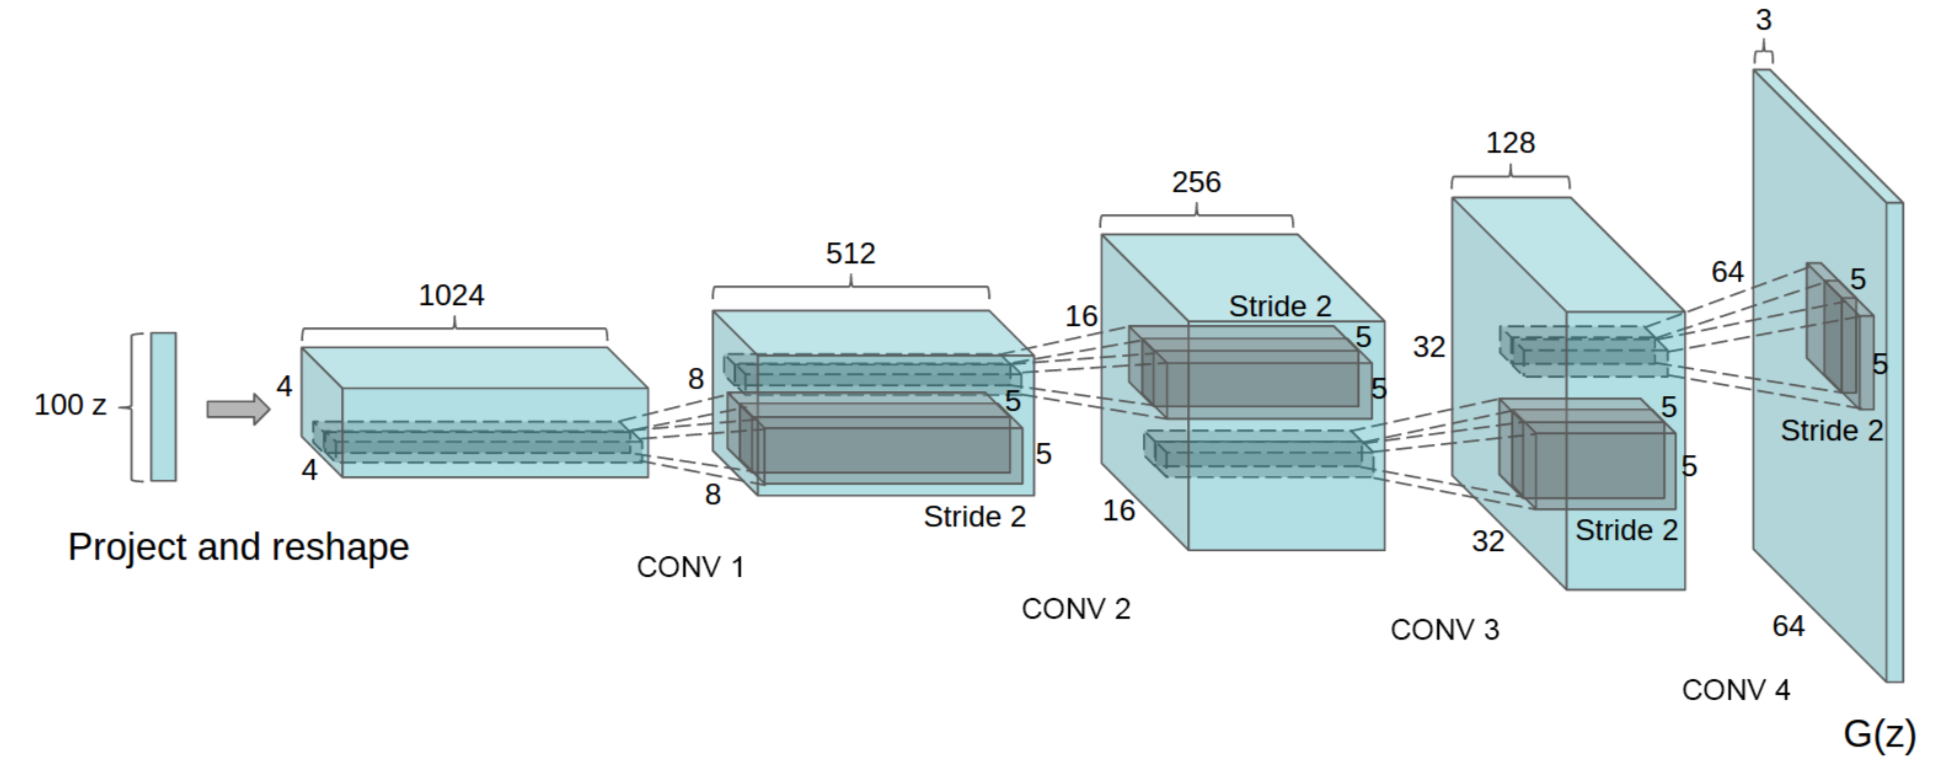
\includegraphics[width=0.7\textwidth]{images/cgan_architecture}
 \caption[Struktura generatorja uporabljenega v \cite{antipov2017face}]{Struktura generatorja uporabljenega v \cite{antipov2017face}.\\Vir: \cite{radford2015unsupervised}}
  \label{fig:agecgan-generator}
\end{figure}

Ker sta tako generator $G(z,y)$ kot nevronska mreža $FR$ odvedljiva glede na vhodne podatke, potem se optimizacijo lahko rešuje z uporabo \textbf{L-BFGS-B} algoritma, ki mu kot začetni približek podamo vrednost $z_0$, ki smo jo dobili iz enkoderja $E$. 
\subsection{Staranje z uporabo ponavljajočih nevronskih mrež}
Klasične ponavljajoče nevronske mreže podajajo dobre rezultate, kadar se ukvarjamo z zaporednimi podatki, kjer so členi medsebojno odvisni, to pa lahko izkoristimo za simuliranje postopka staranja \cite{wang2016recurrent}
Staranje si lahko predstavljamo kot zaporedje stanj, kjer je vsako novo stanje odvisno od prejšnjega. Starosti razdelimo na starostne skupine, cilj pa je najti prehode iz enega stanja v naslednjega. 
Postopek je sestavljen iz dveh glavnih korakov, kjer je prvi normalizacija obraznik slik, drugi pa staranje s pomočjo mreže. 
Pomembno je, da nam normalizacija ohrani podatke o starosti ter lepe prehode med starostnimi skupinami. 
Za dosego tega cilja se poslužimo tehnike, kjer normaliziramo slike sosednih starostnih skupin skupaj. Uporablja se  optični tok, saj  ohrani teksturne podrobnosti na slikah.  Podrobnosti in matematična formulacija  so podrobneje predstavljene  v 
\cite{wang2016recurrent}. 
Ko imamo slike normalizirane, se poslužimo ponavljajoče nevronske mreže, za izvajanje postopka staranja. 
Osnovna komponenta mreže so dvoslojna GRU (gated recurrent unit) vrata, kjer spodnji GRU zakodira vhodni obraz v skrito visokodimenzionalno reprezentacijo, ki jo zgornji del odkodira v postaran obraz. Kot našo kriterijsko funkcijo 
določimo razliko med vhodno sliko in referenčno sliko. Uteži postopoma povečujemo tako, da ima največjo težo razlika med najstarejšo starostno skupino in referenco. S tem omogočimo bolj realne prehode med stanji.



\subsection{Staranje s pogojnim nasprotniškim autoenkoderjem}
Predpostavimo da slike oseb pri različnih starostih ležijo na mnogoterosti $\mathcal{M}$. Premikanje po tem prostoru v določeni smeri nam ohrani identiteto, kljub temu da se starost spreminja. Želimo določiti 
 preslikavo med nižjedimenzionalnim latentnim prostorom in mnogoterostjo, saj je direktna preslikava med sliko in mnogoterstjo pretežka za modeliranje. 
 \\ 
 Imamo sliko obraza $x$, ki jo enkoder $E$ preslika v latentno reprezentacijo $z$, ki jo nato združimo z informacijo o starosti osebe $l$. S tem dobimo točko na $\mathcal{M}$. Glavna ideja je, da sta v latentnem prostoru informaciji o identiteti $z$ in starosti $l$ ločeni. To pomeni, da lahko samo spremenimo starost in s tem ohranimo identiteto osebe. S pomočjo generatorja $G$ to preslikamo nazaj v prostor slik, ki so človeku berljive. 
Za enkoder uporabimo konvolucijsko nevronsko mrežo, kjer se za namene downsamplinga (?) uporablja koračenje s korakom 2, kot je priporočeno v \cite{radford2015unsupervised}. Podobno velja za generator. 
Imamo tudi dva diskriminatorja: 
\begin{itemize}
\item $D_z$ je povezan z enkoderjem in skrbi, da latentni vektorji $z$ sledijo normalni porazdelitvi. S tem želimo prisiliti $E$ da je latentni prostor enakomerno zapolnjen.
\item $D_{img}$ prisili generator, da so rezultati fotorealistični, še posebej  se to vidi pri teksturi starejših obrazov.  
\end{itemize}

Pri podanem latentnem vektorju $z$ ter oznaki $l$, nam generator $G$ ustvari novo sliko $\hat{x} = G(z,l) = G(E(x),l)$. Želimo, da $\hat{x}$ leži na na $\mathbb{M}$ in ima isto identiteto kot $x$. 
Matematično je naš  cilj  dobiti rešitev enačbe 
$$ \min_{E,G} \mathcal{L}(x,G(E(x),l))$$. 
 ter hkrati posrbeti, da je $z$ normalno porazdeljen ter da je kriterij diskriminatorja $D_{img}$ čim bolj izpolnjen.\\
 Porazdelitev učnih podatkov definiramo kot $p_{data}(x)$ in porazdelitev $z$ definiramo kot $q(z|x)$. Naj bo $p(z)$ priorna porazdelitev, potem z $z^* \sim p(z)$ definiramo vzorčenje iz $p(z)$. 
 Skupno učenje $E$ in $D_z$ predstavimo s kriterijsko funkcijo 
 $$ \min_E \max_{D_z}\mathbb{E}_{z^* \sim p(z)}[\log{D_z(z^*)}] + \mathbb{E}_{x \sim p_{data}(x)}[log(1-D_z(E(x)))]$$.
 Analogno lahko definiramo kriterijsko funkcijo za učenje diskrimanatorja $D_{img}$ in generatorja $G$ z oznako $l$ kot  
 $$ \min_G \max_{D_{img}} \mathbb{E}_{x,l \sim p_{data}(x,l)}[\log{D_{img}(x,l)}] + \mathbb{E}_{x,l \sim p_{data}(x,l)}[\log(1-D_{img}(G(E(x),l)))] $$

Vse skupaj sedaj seštejmo in združimo v celotno kriterijsko funkcijo sistema

\begin{equation}
\begin{aligned}
 \min_{E,G} \max{D_z,D_{img}} \lambda \mathcal{L}(x,G(E(x),l))   \\
+ \mathbb{E}_{z^* \sim p(z)}[\log{D_z(z^*)}]  \\
+ \mathbb{E}_{x \sim p_{data}(x)}[log(1-D_z(E(x)))]   \\
+ \mathbb{E}_{x,l \sim p_{data}(x,l)}[\log{D_{img}(x,l)}]  \\ 
+ \mathbb{E}_{x,l \sim p_{data}(x,l)}[\log(1-D_{img}(G(E(x),l)))]
\end{aligned}
\end{equation}


\section{Osnovni generativni modeli}
\subsection{Autoenkoder}
Ena od glavnih arhitektur na področju generativnih modelov je autoenkoder. Avtoenkoderji so sestavljeni iz dveh glavnih delov, \textbf{enkoderja} $E$ in \textbf{dekoderja} $D$. 
Cilj enkoderja je stisniti vhodne podatke v latentno reprezentacijo manjše dimenzije, cilj dekoderja pa je iz latente reprezentacije rekonstruirati vhodne podatke. 
Želimo torej $$ E(x) = y \text{ in } D(y) \approx x $$ 

\begin{figure}[ht]
  \centering
  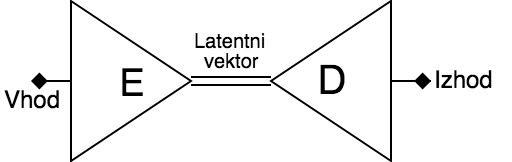
\includegraphics[width=0.35\textwidth]{images/autoencoder_schema.png}
 \caption[Idejna shema oblike autoenkoderja]{Idejna shema oblike autoenkoderja.}
  \label{fig:autoencoder-shape}
\end{figure}

V splošnem se bo v procesu kodiranja in odkodiranja vedno zgodila izguba informacij, saj je latentni prostor manjše dimenzije kot vhodni podatek. Naprimer, sliko velikost 28x28 točk stisnemo v vektor velikost 10x1. 
\\
Nevronsko mrežo učimo tako, da želimo da je rekonstuiran podatek čim bolj podoben vhodnemu. Na prvi pogled se zdi, da je uporabnost avtoenkoderjev omejena na kompresijo podatkov, vendar obstaja velika uporabnost na področju generativnih modelov. 
Ker je latentni prostor manjše dimenzije, prisilimo mrežo, da v latentni prostor zakodira čim več informacije in tako ohrani najpomembnejše značilke na slikah. \\
V praksi je to koristno v namene razšumljanja slik, inpaintinga. V teh primerih mrežo naučimo da iz nepopolnih (manjkajočih, šumnatih) slik zgenerira čiste slike. 
\\
V najbolj enostavni obliki je autoenkoder sestavljen iz treh slojev. Vhodni sloj je polno povezav z edinim skritim slojem, ki je nato polno povezan z izhodnim slojem. 
V praksi je najpogostejša izboljšava osnovne arhitekture  oblika z več polnopovezanimi skritimi sloji, ki se zmanjšujejo v velikosti na strani enkoderja in povečujejo na strani dekoderja. 
Če delamo s podatki kot so slike, lahko polnopovezane sloje zamenjamo s konvolucijskimi sloji različnih velikosti. 
\\
Dimenzije skritih slojev in latentnega vektorja so odvisne od dimenzij vhodnih podatkov ter od tipa podatkov s katerimi delamo. Parametri modela morajo biti prilagojeni našim podatkom in cilju, ki ga želimo doseči. 

\begin{figure}[ht]
  \centering
  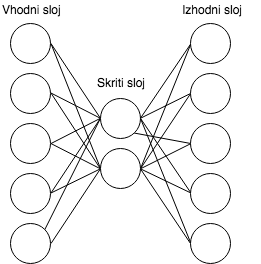
\includegraphics[width=0.35\textwidth]{images/autoencoder.png}
 \caption[Diagram najenostavnejšega autoenkoderja]{Diagram najenostavnejšega autoenkoderja.}
  \label{fig:autoencoder-diagram}
\end{figure}


\subsection{Generativne nasprotniške mreže}
Generativne nasprotniške mreže so bile prvič predstavljene v članku  \cite{gangoodfellow}, kjer je predstavljen algoritem tudi podkrepljen s teoretičnimi
dokazi. Glavna ideja algoritma je, da pomerimo generativni model proti nasprotniku, ki določa ali je generiran rezultat podoben tistemu, ki ga želimo modelirati. 
Predstavljamo si lahko bitko med ponarejevalcem denarja in strokovnjakom, ki določa ali je kos denarja pristen. Želimo, da oba akterja skozi iterativni nasprotniški proces izboljšujeta drug drugega. \\ I
dejno shemo  mreže lahko vidimo na sliki \ref{fig:gan-diagram}. To lahko primerjamo s shemo autoenkoderja  \ref{fig:autoencoder-shape} in razlike v arhitekturi so očitne. 
\begin{figure}[ht]
  \centering
  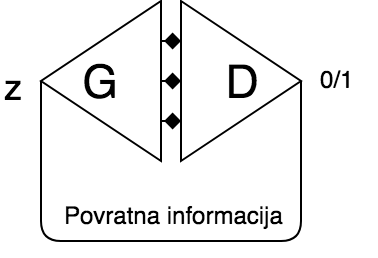
\includegraphics[width=0.35\textwidth]{images/gan_schema.png}
 \caption[Diagram strukture autoenkoderja ]{Generator na vhod dobi šum $z$ iz katerega zgenerira rezultat, diskriminator pa pove ali misli, da je slika iz učne množice ali ne}
  \label{fig:gan-diagram}
\end{figure}


Rečemo, da sta oba  diskriminator kot generator večslojni nevronski mreži. Matematično gledano, želimo naučiti generator G, da bo proizvajal vzorce, katerih porazdelitev je podobna porazdelitvi podatkov, katere želimo modelirati. Da bi se naučili porazdelitev generatorja $p_g$ na podatkih $x$, definiramo priorni porazdelitev $p(z)$, kjer $z$ predstavlja vektor šuma.\\ Preslikavo v prostor podatkov predstavimo z $G(z;\theta_g)$, kjer je G odvedljiva funkcija, ki jo predstavlja večslojna nevronska mreža in $\theta_g$ njeni parametri.  Prav tako definiramo $D(x,\theta_d)$, katerega izhod je skalar $D(x)$ ,ki predstavlja verjetnost, da je $x$ prišel iz podatkov in ne iz  $p_g$ (torej ni bil generiran s pomočjo generatorja). Hočemo torej, da diskriminator za vhod vedno pravilno določi ali je prišel iz množice realnih podatkov oz. ali je bil generiran s pomočjo generatorja $G$. To zapišemo kot: 
\begin{equation}
\label{eq:gan-main}
 \min_G\max_DV(D,G) = \mathbb{E}_{x \sim p_{data}(x)}[\log{D(x)}] + \mathbb{E}_{z \sim p_z(z)}[\log{(1-D(G(z)))]} 
\end{equation}

Psevdokoda algoritma, ki uporablja gradientni spust za implementacijo našega generativnega nasprotniškega modela, je sledeča: 
\begin{algorithm}
\caption{Učenje generativnega nasprotniškega modela s pomočjo gradientnega spusta}\label{euclid}
\begin{algorithmic}[1]
\For{št. iteracij treninga}
\For{$k$ korakov}
	\State {Vzorči $m$ vzorcev  $ \{ z^{(1)},\dots ,z^{(m)} \} $ iz priorne porazdelitve $p_g(z)$}
	\State {Vzorči $m$ vzorcev  $ \{ x^{(1)},\dots,x^{(m)} \} $ iz porazdelitvne podatkov $p_{data}(x)$ } 
	\State {Posodobi diskriminator z vzpenjanjem po gradientu
				$$ \nabla \theta_d \frac{1}{m}\sum_{i=1}^{m}[\log{D(x^{(i)})} + \log{(1-D(G(z^{(i)}))}] $$}
\EndFor
	\State {Vzorči $m$ vzorev  $ \{ z^{(1)},\dots ,z^{(m)} \} $ iz priorne porazdelitve $p_g(z)$ }
	\State {Posodobi generator s pomočjo gradientnega spusta
				$$ \nabla \theta_d \frac{1}{m} \sum_{i=1}{m}\log{(1-D(G(z^{(i)})))}$$}
\EndFor
\end{algorithmic}
\end{algorithm}

Parameter $k$ za število iteracij notranje zanke, določimo glede na eksperimentalne korake. Pove nam kolikokrat naredimo korak optimizacije diskriminatorja za vsak korak generatorja. 
Želimo, da generator in diskriminator ostajata v ravnovesju. Če eden od njiju postane preveč učinkovit, težko pride do nadaljnjega izboljšanja v kvaliteti rezultatov, kar je tudi ena glavnih slabosti tega pristopa.  
Na začetku učenja, ko je G slab, se v praksi lahko zgodi, da $D$ z lahkoto zavrne vse generirane vzorce, saj so očitno različni od podatkov iz učne množice. V tem primeru se vrednost $\log(1-D(G(z)))$ močno poveča in težko najdemo globalni minimum. Da se izognemo temu problemo, reformuliramo problem tako, da namesto minimizacije  $\log(1-D(G(z)))$ učimo $G$, da maksimizira $\log{D(G(z))}$. To nam omogoča. da na začetku učenja dobimo močnešje gradiente, ki omogoča boljše premike v smer optimalne rešitve. 
\\
Ena od možnih razširitev omenjenih v članku je razširitev na pogojni generativni model $p(x | c)$, kar  dobimo tako, da dodamo pogoj $c$ na vhod tako generatorju kot diskriminatorju.  


\subsection{Variacijski autoenkoder}
Eden od glavnih pristopov pri generativnem strojnem učenju je uporaba variacijskih autoenkoderjev \cite{kingma2013auto}.  TI so posplošitev autoenkoderja, kjer  enkoder pogojimo da ustvarjeni latentni vektorji okvirno sledijo normalni porazdelitvi. Generiranje novih slik je torej samo vzorčenje iz  normalne porazdelitve,
z določeno srednjo vrednostjo in standardno deviacijo, ki jo dobimo iz mreže. Vedno je potreben kompromis med rekonstrukcijsko napako in prileganjem normalni porazdelitvi. 
Statistično gledano imamo spremenljivko $z$, katera generira $x$. Izračunali bi radi $p(z|x) = \frac{p(x|z)p(z)}{p(x)}$. Izkaše se, da je izračun te porazdelitve v praksi problematičen, zato aproksimiramo to porazdelitev z porazdelitvijo $q(z|x)$, ki ji je podobna in jo znamo izračunati. Za mero podobnosti med dvema porazdelitvama pa uporabimo KL divergenco. 
V naslednjem delu predstavimo bolj natančno in formalno izpeljavo variacijskega autoenkoderja. 
 \\
Predstavljajmo si množico $ X = \{x^{(i)}\}_{i=n}^N$, ki vsebuje $N$ neodvisnih in enakomerno porazdaljenih slučajnih spremenljivk $x$. Predpostavimo, da so podatki generirani s pomočjo nekega naključnega procesa, ki vključuje slučajno spremenljivko $z$, ki pa jo ne vidimo. \\
Ta proces je sestavljen iz dveh korakov 
\begin{enumerate}
\item Vrednost $z^{(i)}$ je generirana iz predhodne porazdelitve $p_{\theta^*}(z)$
\item Vrednost $x^{i}$ je generirana iz pogojne porazdelitve $p_{\theta^*}(x|z)$
\end{enumerate}

Predpostavimo, da $p_{\theta^*}(z)$ in $p_{\theta^*}(x|z)$ prihajata iz družine porazdelitev 
$p_{\theta}(z)$ in $p_{\theta}(x|z)$ in da je njihova gostota verjetnosti povsod odvedljiva glede na parametra $\theta$ in $z$.  
V praksi so vrednosti $z^{(i)}$ ter vrednost $\theta^*$ neznane. \\
Zanima nas rešitev, ki deluje tudi v primeru večje podatkovne množice ter kadar je intergral marginalne verjetnosti 
$p_\theta (x) = \int p_\theta (z)p_\theta (x|z)dz$ neobladljiv ( ne moremo ga odvajati oz. izračunati) in kjer je posteriorna gostota
$p_\theta(z|x) = p_\theta(z|x)p_\theta(z)/p_\theta(x)$ neobvladljiva. Ta dva primera, se velikokrat pojavljata prav v nevronskih mrežah z nelinearnimi skritimi sloji. 
\\
Pristop z variacijskimi autoenkoderji nam omogoča učinkovito ocenjevanje parametrov $\theta$, kar nam omogoča generiranje umetnih podatkov, ki so podobni naravnim. Kadar imamo neko vrednost $x$ ter izbrane parametre $\theta$, nam VAE omogoča 
dobiti aproksimacijo latentne spremenljivke $z$. To se uporablja v namene kodiranja, kjer informacije iz $x$ zakodiramo v $z$. 
Še ena od uporabnih lastnosti pa je aproksimiranje inference spremenljivke $x$, kar nam omogoča uporabo v smeri razšumenja, "inpaintinga" itd. 
\\
Uvedemo prepoznavni model $q_\phi(z|x)$, ki je aproksimacija $p_\theta(z|x)$. Izpeljali bomo metodo, ki se  $\phi$ nauči skupaj s parametri $\theta$
Neopazovano spremenljivko $z$, si lahko predstavljamo kot zakodirano informacijo.  Zato model $q_\phi(z|x)$ imenujemo \textbf{enkoder}, saj nam glede na podatek  $x$ izračuna porazdelitev možnosti $z$, ki bi lahko generirale ta podatek. 
Analogno bomo $p_\theta(x|z)$ imenovali \textbf{dekoder}, saj nam iz $z$ producira porazdelitev čez vrednosti $x$.  
\\
Izpeljemo lahko spodnjo mejo: 
$$ \mathcal{L}(\theta,\phi,x^{(i)}) = - D_{KL}(q_\phi(z|x^{(i)})||p_\theta(z)) + \mathbb{E}_{q\phi (z|x^{(i)})}[\log{p_\theta(x^{(i)}|z)}] $$
ki jo želimo optimizirati glede na parametre $\phi$ in $\theta$.  Zaradi velike variance gradienta, je naivna Monte Carlo metoda, za ta primer neučinkovita in potrebujemo boljšo metodo. 
\\
Zanima nas cenilka za  spodnjo mejo $\mathcal{L}$ in njene odvode. Upoštevajoč nekaj pogojev, ki so bolj natančno razloženi v \cite{kingma2013auto}, lahko reparametriziramo $\tilde{z} \sim q_\phi(z|x)$ z odvedljivo preslikavo šuma $\epsilon$, torej 
$\tilde{z} = g_\phi(\epsilon,x)$, kjer velja $\epsilon \sim p(\epsilon)$.
Sedaj lahko vpeljemo Monte Carlo aproksimacijo za pričakovano frednost neke funkcije $f(z)$, glede na $q_\phi(z|x)$. kot

$$ \mathbb{E}_{q_\phi(z|x^{(i)})}[f(z)] = \mathbb{E}_{p(\epsilon)}[f(g_\phi(\epsilon,x^{(i)}))] \simeq \frac{1}{L}\sum_{l=1}^{L}f(g_\phi(\epsilon^{(l)},x^{(i)})) $$
, kjer je $\epsilon^{(l)} \sim p(\epsilon)$. \\
To tehniko apliciramo na naš problem in dobimo cenilko $\tilde{\mathcal{L}}^A(\theta,\phi;x^{(i)}) \simeq \mathcal{L}(\theta,\phi;x^{(i)})$  za katero velja 

$$  \tilde{\mathcal{L}}^A(\theta,\phi;x^{(i)}) = \frac{1}{L} \sum_{l=1}^L \log{p_\theta (x^({i}),z^{(i,l)})}-\log{q_\phi (z^{(i,l)}|x^{(i)})} $$ kjer 
$$z^{(i,l)} = g_\theta(\epsilon^{(i,l)},x^{(i)}) \text{ in } \epsilon^{(l)} \sim p(\epsilon)$$

Velikokrat lahko $KL-divergenco$ integriramo analitično, tako da je ocena z vzorčenjem potrebna le za rekonstrukcijsko napako. $\mathbb{E}_{q\phi(z|x^{(i)})}[\log{p_\theta(x^{(i)}|z)}$. KL-divergenco si lahko predstavljamo kot regularizacijski člen $\phi$, kar nam 
da drugo različico cenilke $ \widetilde{\mathcal{L}}^B(\theta,\phi;x^{(i)}) \simeq \mathcal{L}(\theta,\phi;x^{(i)}) $ ki je definirana kot 
 $$ \widetilde{\mathcal{L}}^B(\theta,\phi;x^{(i)}) = - D_{KL}(q_\phi(z|x^{(i)})||p_\theta(z)) + \frac{1}{L}\sum_{l=1}^L(\log{p_\theta(x^{(i)}|z^{(i,l)}))} $$ 
in velja $$ z^{(i,l)} = g_\phi(\epsilon^{(i,l)},x^{(i)}) \text{ in }  \epsilon^{(l)} \sim p(\epsilon)$$
\\
Če Iz podatkovnem množice $X$ z $N$ elementi vzorčimo po $M$ vzorcev, lahko skonstruiramo cenilko osnovano na "minibatchih": 
 $$ \mathcal{L}(\theta,\phi;X) \simeq \widetilde{\mathcal{L}}(\theta,\phi;X^M) = \frac{N}{M}\sum_{i=1}^M \widetilde{\mathcal{L}}(\theta,\omega;x^{(i)}) $$ 
Minibatch $X^M = \{ x^{(i)} \}_{i=1}^M$ je naključno izbran vzorec velikosti $M$ iz množice $X$.
V psevdokodi je  algoritem predstavljen kot 
\begin{algorithm}
\caption{Minibatch verzija AEVB algoritma. Lahko se uporablja cenilka $\widetilde{\mathcal{L}}^A$ ali $\widetilde{\mathcal{L}}^B$ }\label{minibatch-aevb}
\begin{algorithmic}[1]
\State $\theta,\phi \leftarrow$  inicializacija parametrov
\Repeat 
	\State $X^M \leftarrow$ Naključen minibatch $M$ vzorcev iz $X$
	\State $\epsilon \leftarrow$ Naključni vzorec šuma iz porazdelitve $p(\epsilon)$
	\State $g \leftarrow \nabla_{\theta,\phi}\widetilde{\mathcal{L}}^M(\theta,\phi;X^M,\epsilon)$ (Gradient minibatch cenilke)
	\State $\theta,\phi \leftarrow$ Posodobimo parametre s premikom v smeri gradienta (SGD ali ADAGRAD)	  
\Until parametra $(\theta,\phi)$ skonvergirata \\
\Return $\theta,\phi$
\end{algorithmic}
\end{algorithm}

\subsection{Nasprotniški autoenkoder}
Nasprotniški autoenkoderji \cite{adverserialautoencoders} so razširitev autoenkoderjev in so po svoje zasnovi precej podobni variacijskim avtoenkoderjem.  
Glavna razlika se pojavi v načinu zagotavljanja porazdelitve latentnega vektorja. Variacijski autoenkoder uporablja KL-divergenco kot vodilo za vodenje pravilne porazdelitve, medtem ko se
pri nasprotniških avtoenkoderjih uporablja nasprotniško učenje, kjer želimo s pomočjo diskriminatorja doseči isti cilj. 
\\
Naj bo $x$ vhodni podatek, $z$ latentni vektor autoenkoderja in $p(z)$ porazdelitev kateri želimo da koda $z$ sledi. Definirajmo $q(z|x)$ kot porazdelitev enkoderja, $p(x|z)$ kot porazdelitev dekoderja, $p_d(x)$ kot porazdelitev podatkov ter 
$p(x)$ kot porazdelitev našega modela. Enkoder definira porazdelitev $q(z)$ na latentnem vektorju kot  $$ q(z) = \int_x q(z|x)p_d(x)dx $$
Nasprotniški autoenkoder je autoenkoder, ki je regulariziran z ujemanjem med $q(z)$ in $p(z)$. \\
Nasprotniška mreža je zadolžena za vodenje porazdelitve $q(z)$ proti $p(z)$, medtem ko je autoenkoder zaslužen za minimiziranje rekonstrukcijske napake. 
Velja, da je generator nasprotniške mreže tudi enkoder autoenkoderja $q(z|x)$, ki je zadolžen da prelisiči diskriminator, da ne loči med $q(z)$ in $p(z)$.
Učenje vedno izvajamo v dveh delih, najprej učimo nasprotniško mrežo (diskriminator) in s tem regulariziramo porazdelitev latentnega vektorja. S tem se posodobi tudi generator mreže, ki je hkrati enkoder autoenkoderja tako, da bolje zmede diskriminator.  V 
drugem koraku pa učimo autoenkoder in s tem izboljšujemo rekonstrukcijsko napako. 
\\
Možnih je nekaj različnih izbir za enkoder $q(z|x)$
\begin{itemize}
\item \textbf{Deterministični} Predpostavimo, da je $q(z|x)$ deterministična funkcija $x$-a. V tem primeru je enkoder podoben enkoderju standardnega autoenkoderja in edini vir stohastičnosti (nepredvidljivosti)  v $q(z)$ ostane učna množica $p_d(x)$.
\item \textbf{Normalno porazdeljeni} Privzamemo, da je $q(z|x)$ normalna porazdelitev, katere srednja vrednost in varianca je dobljena iz enkoderja. Velja torej $$z_i \sim \mathcal{N}(\mu_i(x),\sigma_i(x))$$ V tem primeru stohastičnost dobimo tako iz učne množice kot iz naključnosti naravne porazdelitve.
\item \textbf{Univerzalni aproksimator} To si predstavljamo kot posplošitev prejšne možnosti. Cilj je, da  $q(z|x)$ naučimo kot univerzalni aproksimator. Naj bo enkoder funkcija $f(x,\eta)$, ki na vhod dobi $x$ in  naključni šum $\eta$ s fiksno porazdelitvijo, potem lahko vzorčimo iz katerekoli posteriorne porazdelitve $q(z|x)$, tako da evaluiramo $f(x,\eta)$ pri različnih vzorcih 
$\eta$. Matematično gledano, predpostavimo da velja $q(z|x,\eta)$ = $\delta(z-f(x,\eta))$ in 
$$q(z|x) = \int_{\eta} q(z|x,\eta)p_\eta(\eta)d \eta \implies q(z) = \int_x \int_{\eta} q(z|x,\eta)p_{d}(x)p_{\eta}(\eta)d \eta dx $$ 
Tu je stohastičnost  v $q(z)$ dobljena tako iz učne množice kot iz šuma $\eta$ na vhodu enkoderja. V tem primeru nismo več omejeni na naravno porazdelitev, ampak si lahko izberemo kakršnokoli porazdelitev želimo, saj to določuje porazdelitev šuma $\eta$. 
\end{itemize}

Nasprotniški autoenkoder je mogoče razširiti v pogojno obliko kjer vsem učnim vzorcem dodelimo oznako kateremu razredu pripadajo. 
Na vhod diskriminatorja dodamo one-hot (?) oznako, ki predstavlja razred, kateremu vzorec pripada. 
Ko enkoder izračuna latentni vektor združimo oznako skupaj s latentnim vektorjem in to podamo dekodirnemu delu mreže. 

\section{Preizkušeni pristopi}
Med raziskovanjem načina za doseganje najboljših rezultatov staranja in pomlajevanja smo se poslužili različnih pristopov, ki jih bomo predstavili v tem poglavju. Predstavili bomo teoretično podlago vsakega od njih ter dosežene rezultate. Analizirali bomo pomanjkljivosti in težave pri implementaciji.  
\\
Za implementacijo različnih modelov, je bila uporabljena programska knjižnica \textbf{Keras 2.0.0}, ki v ozadju uporablja \textbf{Tensorflow 1.0.0}. Za doseganje enakovrednih rezultatov je verzija pomembna, saj lahko starejše ali novejše različice dajejo bistveno drugačne rezultate. 
\\
V vseh poizkusih, razen tam kjer je specifično navedeno drugače, smo za učno množico uporabljali bazo slik  UTKFace \cite{utkface}, ki vsebuje 20000 slik oseb različnih etničnih izvorov, spola ter starosti. Slike v bazi so obrezane ter poravnane ter vsebujejo slike oseb pri različnih osvetlitvah, obraznih mimikah ter stopnjah pokritosti. 

\subsection{Pogojni Wasserstein GAN}
Eden od prvih preizkušenih modelov je bila pogojna različica wasserstein GAN \cite{arjovsky2017wasserstein} modela. Eden od glavnih izzivov pri učenju GAN modelov je nastabilnost učenja, kar pa naj bi wassersteinova različica odpravila. 
\subsubsection{Teoretično ozadje}
Pri učenju generativnih modelov predpostavimo, da podatki prihajajo iz neke porazdelitve,  katere aproksimacijo $P_\theta$ se želimo naučiti.  Da to dosežemo, lahko definiramo slučajno spremenljivko $Z$, ki ima fiksno porazdelitev $p(z)$. To  lahko s pomočjo nevronske mreže (parametrične funkcije) preslikamo v novo slučajno spremenljivko, ki generira vzorce s porazdelitvijo $P_\theta$.
$$ g_\theta : \mathcal{Z} \leftarrow \mathcal{X}$$ 
S spreminjanjem parametrov $\theta$, lahko dosežemo da se $P_\theta$ približna porazdelitvni podatkov $P_r$. 
Želimo izbrati pravilno metriko za definiranje  razdalje med dvema porazdelitvama. 
Obstaja nekaj standardnih možnosti, ki jih lahko uporabimo: 

\begin{itemize}
\item \textbf{TV razdalja}
$$ \delta(\mathbb{P}_r,\mathbb{P}_g) = \sup_{A \in \Sigma} | \mathbb{P}_r(A) - \mathbb{P}_g(A)| $$
\item \textbf{KL divergenca}
$$ KL(\mathbb{P}_r || \mathbb{P}_g) = \int \log{(\frac{P_r(x)}{P_g(x)})}P_r(x)d\mu(x)$$
Kjer je največja težava asimetričnost, torej $KL(\mathbb{P}_r || \mathbb{P}_g) \neq KL(\mathbb{P}_g || \mathbb{P}_r )$ ter 
dejstvo, da je mera neskončna, kadar velja $P_g(x) = 0$ in $P_r(x) > 0$. To nam lahko povzroča težave v začetnih fazah učenja nevronske mreže. 
\item \textbf{Jensen-Shannon (JS) divergenca}
$$ JS(\mathbb{P}_r,\mathbb{P}_g) = KL(\mathbb{P}_r || \mathbb{P}_m) + KL(\mathbb{P}_g || \mathbb{P}_m)$$
kjer je $\mathbb{P}_m$ enak $\mathbb{P}_r + \mathbb{P}_g)/2$. To nam  odpravi  največje pomanjkljivosti KL divergence, saj je simetrična ter  vedno manjša od neskončnosti, saj lahko izberemo $\mu = \mathbb{P}_m$
\item \textbf{EM oz. Wasserstein-1 razdalja}
$$ W(\mathbb{P}_r,\mathbb{P}_g) = \inf_{\gamma \in \Pi(\mathbb{P}_r,\mathbb{P}_g) }\mathbb{E}_{(x,y) \sim \gamma} [||x-y||]$$
kjer nam $\Pi(\mathbb{P}_r,\mathbb{P}_g)$ predstavlja množico vseh skupnih porazdelitev $\gamma(x,y)$, katerih "marginala" sta $\mathbb{P}_r$ in $\mathbb{P}_g$.  Lahko si predstavljamo kot koliko mase mora biti prestavjene da iz ene porazdelitve dobimo drugo. 
\end{itemize}

Izkaže se, da je za nas najbolj zanimiva $EM$ razdalja, saj določena enostavna zaporedja porazdelitev konvergirajo glede na to razdaljo in ne glede na druge. V tej obliki te razdalje ni mogoče izračunati, vendar po Kantarevich-Rubensteinovi dualnosti  je zgornja definicija EM razdalje ekvivalentna 

$$ W(P_r,P_\theta) = \sup_{||f||_L \leq 1 } \mathbb{E}_{x \sim P_r} [f(x)] - \mathbb{E}_{x \sim P_\theta}[f(x)]$$ 

kjer supremum gledamo glede na vse 1-Lipschitz funkcije. Naj bosta $d_x$ in $d_y$ funkciji razdalje definirani na prostorih $X$ in $Y$. Funkcija $f$ je \textbf{K-Lipschitzova} če $\forall x_1,x_2 \in X$ velja $d_y(f(x_1),f(x_2)) \leq Kd_X(x_1,x_2)$.

Psevdokoda WGAN učenja se zapiše kot

\begin{algorithm}
\caption{WGAN algoritem.}\label{wgan-pseudo}
\begin{algorithmic}[1]
\Require $ \alpha $ hitrost učenja, $c$ parameter rezanja, $m$ velikost batcha, $n_{kritik}$ število iteracij kritika na število iteracij generatorja
\Require $w_0$ začetne uteži kritika, $\theta_0$ začetne uteži generatorja
\While{$\theta$ ne skonvergira}
	\For{$t=0,\dots,n_{kritik}$}
		\State Vzorči $\{x^{(i)} \}_{i=1}^m \sim \mathbb{P}_r$ iz učnih podatkov
		\State Vzorči $\{z^{(i)} \}_{i=1}^m \sim p(z)$ iz prejšnje (prior) porazdelitve
		\State $g_w \leftarrow \nabla_w [\frac{1}{m} \sum_{i=1}^m f_w({x^{(i)}})  - \frac{1}{m}\sum_{i=1}^m f_w (g_\theta(z^{(i)}))]$
		\State $w \leftarrow w + \alpha \cdot \text{RMSProp}(w,g_w)$
		\State $w \leftarrow \text{obreži}(w,-c,c)$
	\EndFor
	\State Vzorči $\{z^{(i)}\}_{i=1}^m \sim p(z)$ iz prejšnje (prior) porazdelitve
	\State $g_\theta \leftarrow -\nabla_\theta \frac{1}{m} \sum_{i=1}^m f_w(g_\theta(z^{(i)}))$
	\State $\theta \leftarrow \theta - \alpha \cdot \text{RMSProp}(\theta,g_\theta)$
\EndWhile

\end{algorithmic}
\end{algorithm}

Izkaže se \cite{arjovsky2017wasserstein}, da je za doseganje Lipschnitzovega pogoja dovolj, da funkcije obrežemo (clip) med dve možni vrednosti, ki jih nastavimo s parametrom $c$, kar moramo storiti po vsaki posodobitvi uteži $w$. 
\subsubsection{Eksperimentalni rezultati}

Za doseganje staranja s pomočjo WGAN modela, smo želeli najprej preizkusiti WGAN kot klasični pogojni generativni model. Želeli smo, da bi mreža glede na vhodni šumni vektor ter oznako starosti ustvarila osebo, ki deluje dovolj stara. 
Preizkusili smo dve standardni arhitekturi za obliko generatorja in diskriminatorja. 
Prva arhitektura je bila konvolucijska in je sledila predlogom iz \cite{radford2015unsupervised}. 
Želeli smo mrežo najprej preizkusiti na enostaven način, zato smo se odločili za velikost slike \textbf{64x64} slikovnih točk ter za enokanalne slike. Vsakega od različnih modelov, smo učili za dolžino 20000 batchov. 
\\ Pri konvolucijskem modelu, smo dobili dobili rezultate, ki so prikazani na sliki \ref{fig:cwgan-conv-results}. 
\begin{figure}[ht]
  \centering
  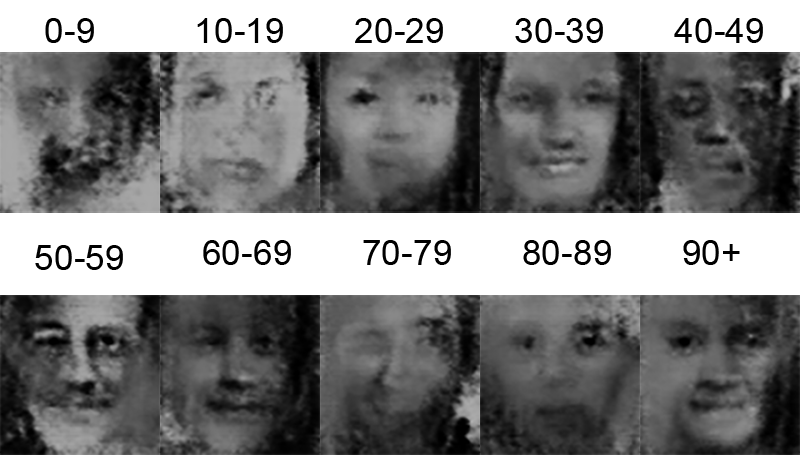
\includegraphics[width=0.5\textwidth]{images/cwgan_conv_results.png}
 \caption[Rezultati učenja CWGAN mreže s konvolucijsko arhitekturo ]{Rezultati učenja CWGAN mreže z konvolucijsko arhitekturo}
  \label{fig:cwgan-conv-results}
\end{figure}
Vidimo, da  je bila naša mreža učena na  učni množici obraznih slik, vendar rezultati niso sprejemljivi, saj so slike zamazane in polne artefaktov. Prav tako so starostni razredi slabo naučeni, saj večina obrazov na slikah na pogled ne pripada pravilni starostni skupini. 
V sklopu učenja smo uporabljali \textbf{RMSProp} optimizator z nastavljeno hitrostjo učenja kot $0.0005$. Parameter rezanja je bil standardno nastavljen na (-1,1) ter $n_{kritik} =5 $. Velikost batch-a pa smo nastavili na $32$. Začetne uteži so bile inicializirane z vzorčenjem iz normalne porazdelitve. 
Razlog za slab uspeh učenja lahko najdemo na grafu vrednosti kriterijske funkcije, ki je viden na sliki \ref{fig:cwgan-loss-graph}

\begin{figure}[ht]
  \centering
  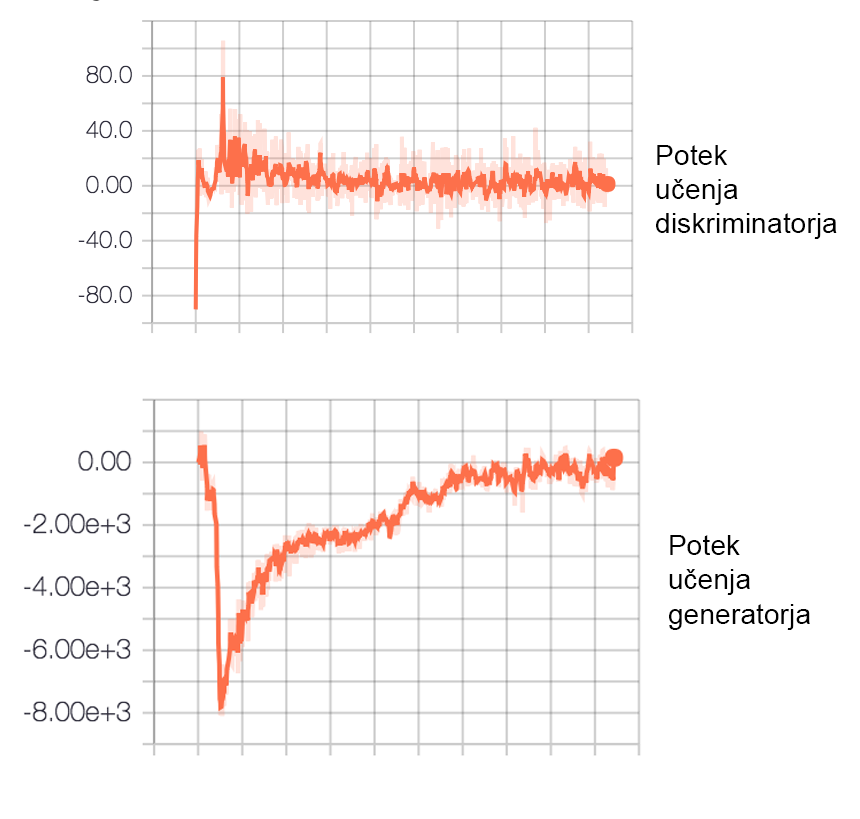
\includegraphics[width=0.5\textwidth]{images/loss_graph_wgan_conv.png}
 \caption[Kriterijska funkcija pri učenju konvolucijskega CWGAN modela ]{Kriterijska funkcija pri učenju konvolucijskega CWGAN modela}
  \label{fig:cwgan-loss-graph}
\end{figure}

Opazimo, da nam diskriminator zelo hitro skonvergira v okolico ničle, vendar se nato tam ne ustali. V času učenja  skače po okolici, kar pomeni, da ne pride do nekih večjih vizualnih izboljšanj. Generator pa  na začetku učenja dobi izrazito negativno vrednost svoje kriterijske funkcije in se nato počasi približuje ničli, a se tudi on tam ne ustali. \\
Da bi izboljšali rezultate, smo poskušali z empiričnim spreminjanjem hiperparametrov (hitrost učenja, $n_{kritik}$, velikost batch-a, število filtrov v konvolucijskih slojih ipd. Prav tako smo poskušali dodati Dropout sloj \cite{srivastava2014dropout} z različnimi parametri, vendar se rezultati niso vidno izboljšali. 
\\
Preizkusili smo tudi uporabo CWGAN arhitekture  s polnopovezanimi sloji, kjer generator s pomočjo zaporednih kaskadnih slojev iz vektorja šuma zgenerira sliko, diskriminator pa samo z uporabo le-teh presodi ali je slika prišla iz množice realnih podatkov ali ne. 
\\Za začetek smo uporabili iste parametre za učenje kot pri konvolucijskem modelu, a smo žal dobili rezultate, ki so bili še manj kvalitetni. Po končanem učenju je večino slik vsebovalo le naključni šum, kar je vidno na sliki \ref{fig:cwgan-dense-imgs}. 

\begin{figure}[ht]
  \centering
  
\includegraphics[width=0.2\textwidth]{images/cwgan_dense_noise.png}
 \caption[Vzorec generiranih slik pri CWGAN modelu s polnopovezanimi sloji]{Vzorec generiranih slik pri CWGAN modelu s polnopovezanimi sloji}
  \label{fig:cwgan-dense-imgs}
\end{figure}


Če pogledamo potek učenja na sliki \ref{fig:cwgan-dense-loss-graph},

\begin{figure}[ht]
  \centering
  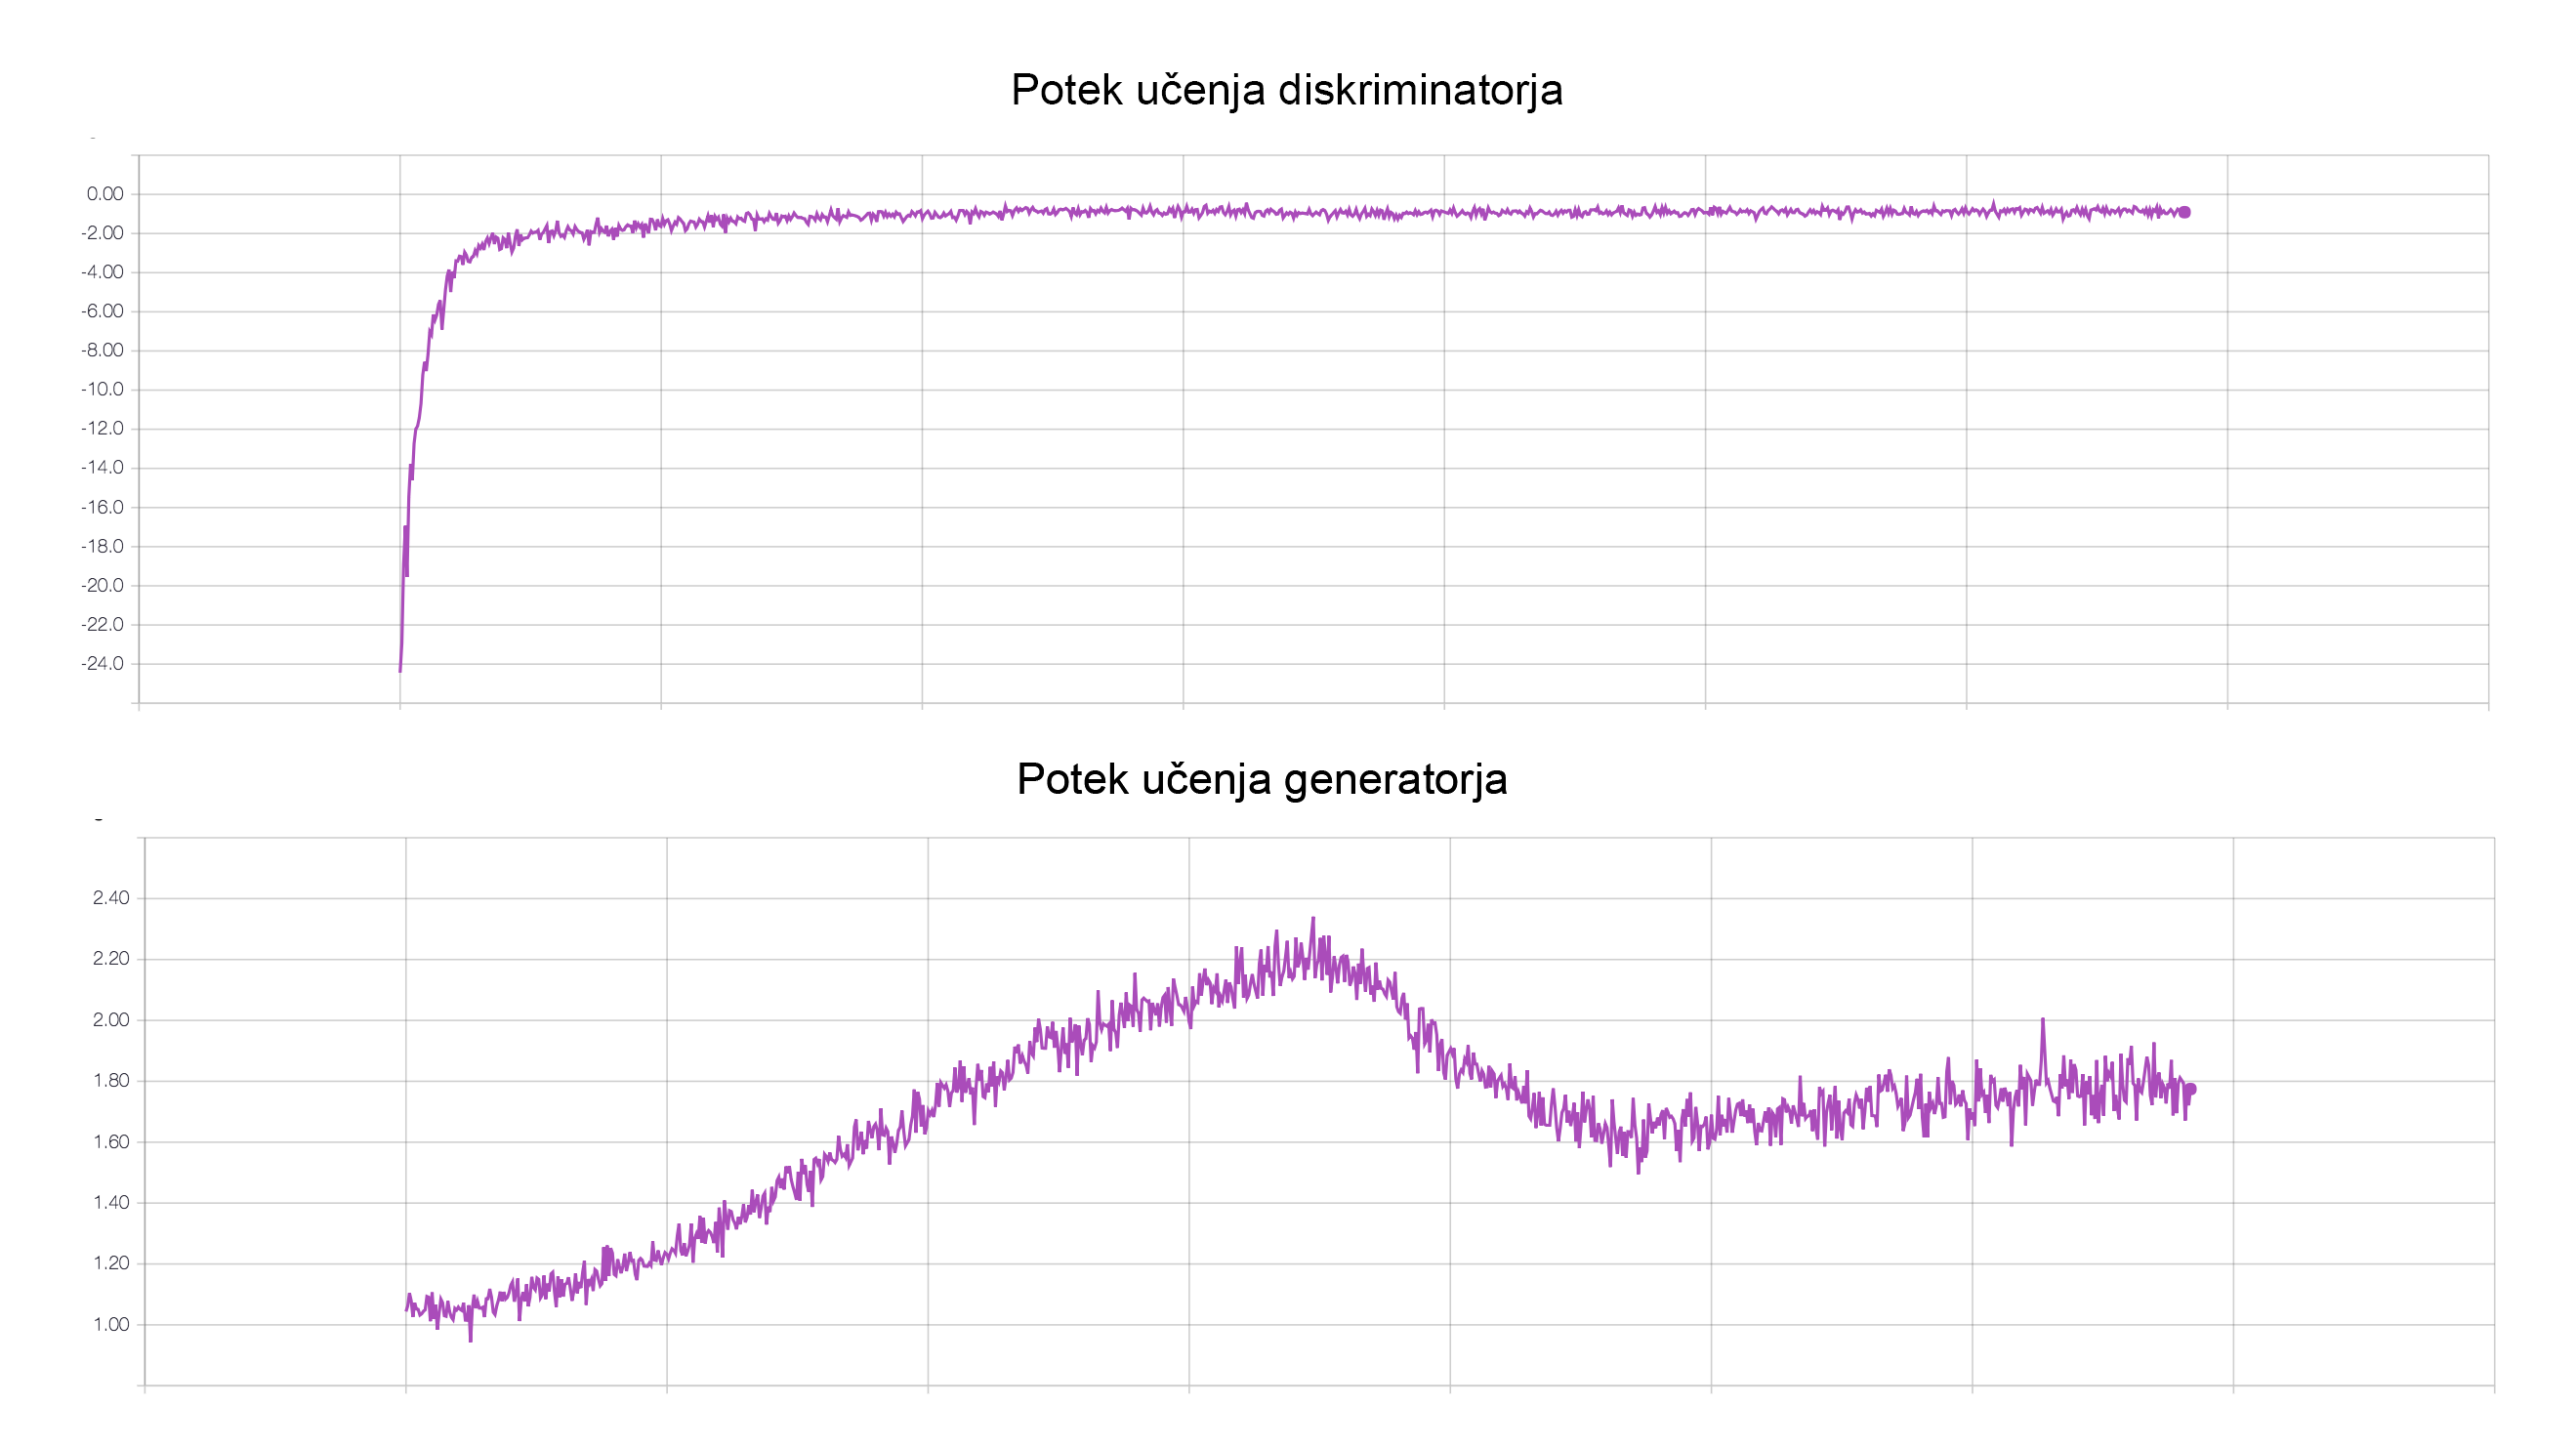
\includegraphics[width=0.8\textwidth]{images/cwgan_dense_loss_graph.png}
 \caption[Kriterijska funkcija pri učenju CWGAN modela s polnopovezanimi sloji ]{Kriterijska funkcija pri učenju CWGAN modela s polnopovezanimi sloji}
  \label{fig:cwgan-dense-loss-graph}
\end{figure}
lahko vidimo da je v tem primeru diskriminator zelo hitro skonvergiral proti optimalni vrednosti 0, medtem ko kriterijska funkcija generatorja ni skonvergirala. To nam lepo prikaže najbolj klasično težavo pri učenju GAN-ov  in sicer neravnovesje v moči med diskriminatorjem  $D$  in generatorjem $G$. V tem primeru je $D$ postal tako dober, da ga $G$, ni znal prelisičiti in medsebojno učenje ni bilo uspešno. Poskusili smo z empiričnim spreminjanjem parametrov, da bi izboljšali rezultate učenja, vendar nam to ni uspela. 

\subsection{BiCOGAN}
\subsubsection{Teoretično ozadje}
Klasični GAN modeli nam omogočijo dobiti preslikavo iz prostora šuma $z$ v prostor generiranih podatkov $x$, vendar v procesu očenja žal ne dobimo obratne preslikave $x \mapsto z$, kar je v določenih primerih zaželjeno, saj nam omogoča dobiti kompaktno reprezentacijo naše informacije $x$. 
\\
Rešitev tega problema je model, ki  pogojno generativno nasprotniško mrežo poveže z enkoderjem. ki je zadolžen za določanje inverzne preslikave \cite{jaiswal2017bidirectional}. Velja \cite{donahue2016adversarial}, da v idealnem primeru morata biti $G$ in $E$ inverzna, da lahko prelisičita diskriminator $D$.
\\
V tem primeru primeru se GAN enačba, zapisana v \ref{eq:gan-main} spremeni v
$$ \min_{G}  \max_{D} V(D,G) = \mathbb{E}_{x \sim p_{data}(x)}[\log{D(x,c)}] + \mathbb{E}_{z \sim p_{\tilde{z}}(\tilde{z})}[\log{(1-D(G(\tilde{z},c))}]$$
\\
Nas so take mreže zanimale zato, saj bi lahko postopek iz \cite{antipov2017face} poenstovali tako, da bi bila potrebna uporaba samo ene nevronske mreže. Pri omenjenem pristopu, so za določanje preslikave iz prostora slik v prostor latentnih vektorjev, uporabili dodatno nevronsko mrežo, kar pa zahteva izgradnjo dodatnega modela ter učenja, ki je ločen od generiranja slik. 
\\
Želja je bila, da bi z uporabo dvosmernega učenja, hkrati učili tako generator in diskriminator kot tudi enkoder. 
Idejno arhitekturo naše mreže v shematski obliki vidimo na \ref{fig:bicogan-archi}. 
\begin{figure}[ht]
  \centering
  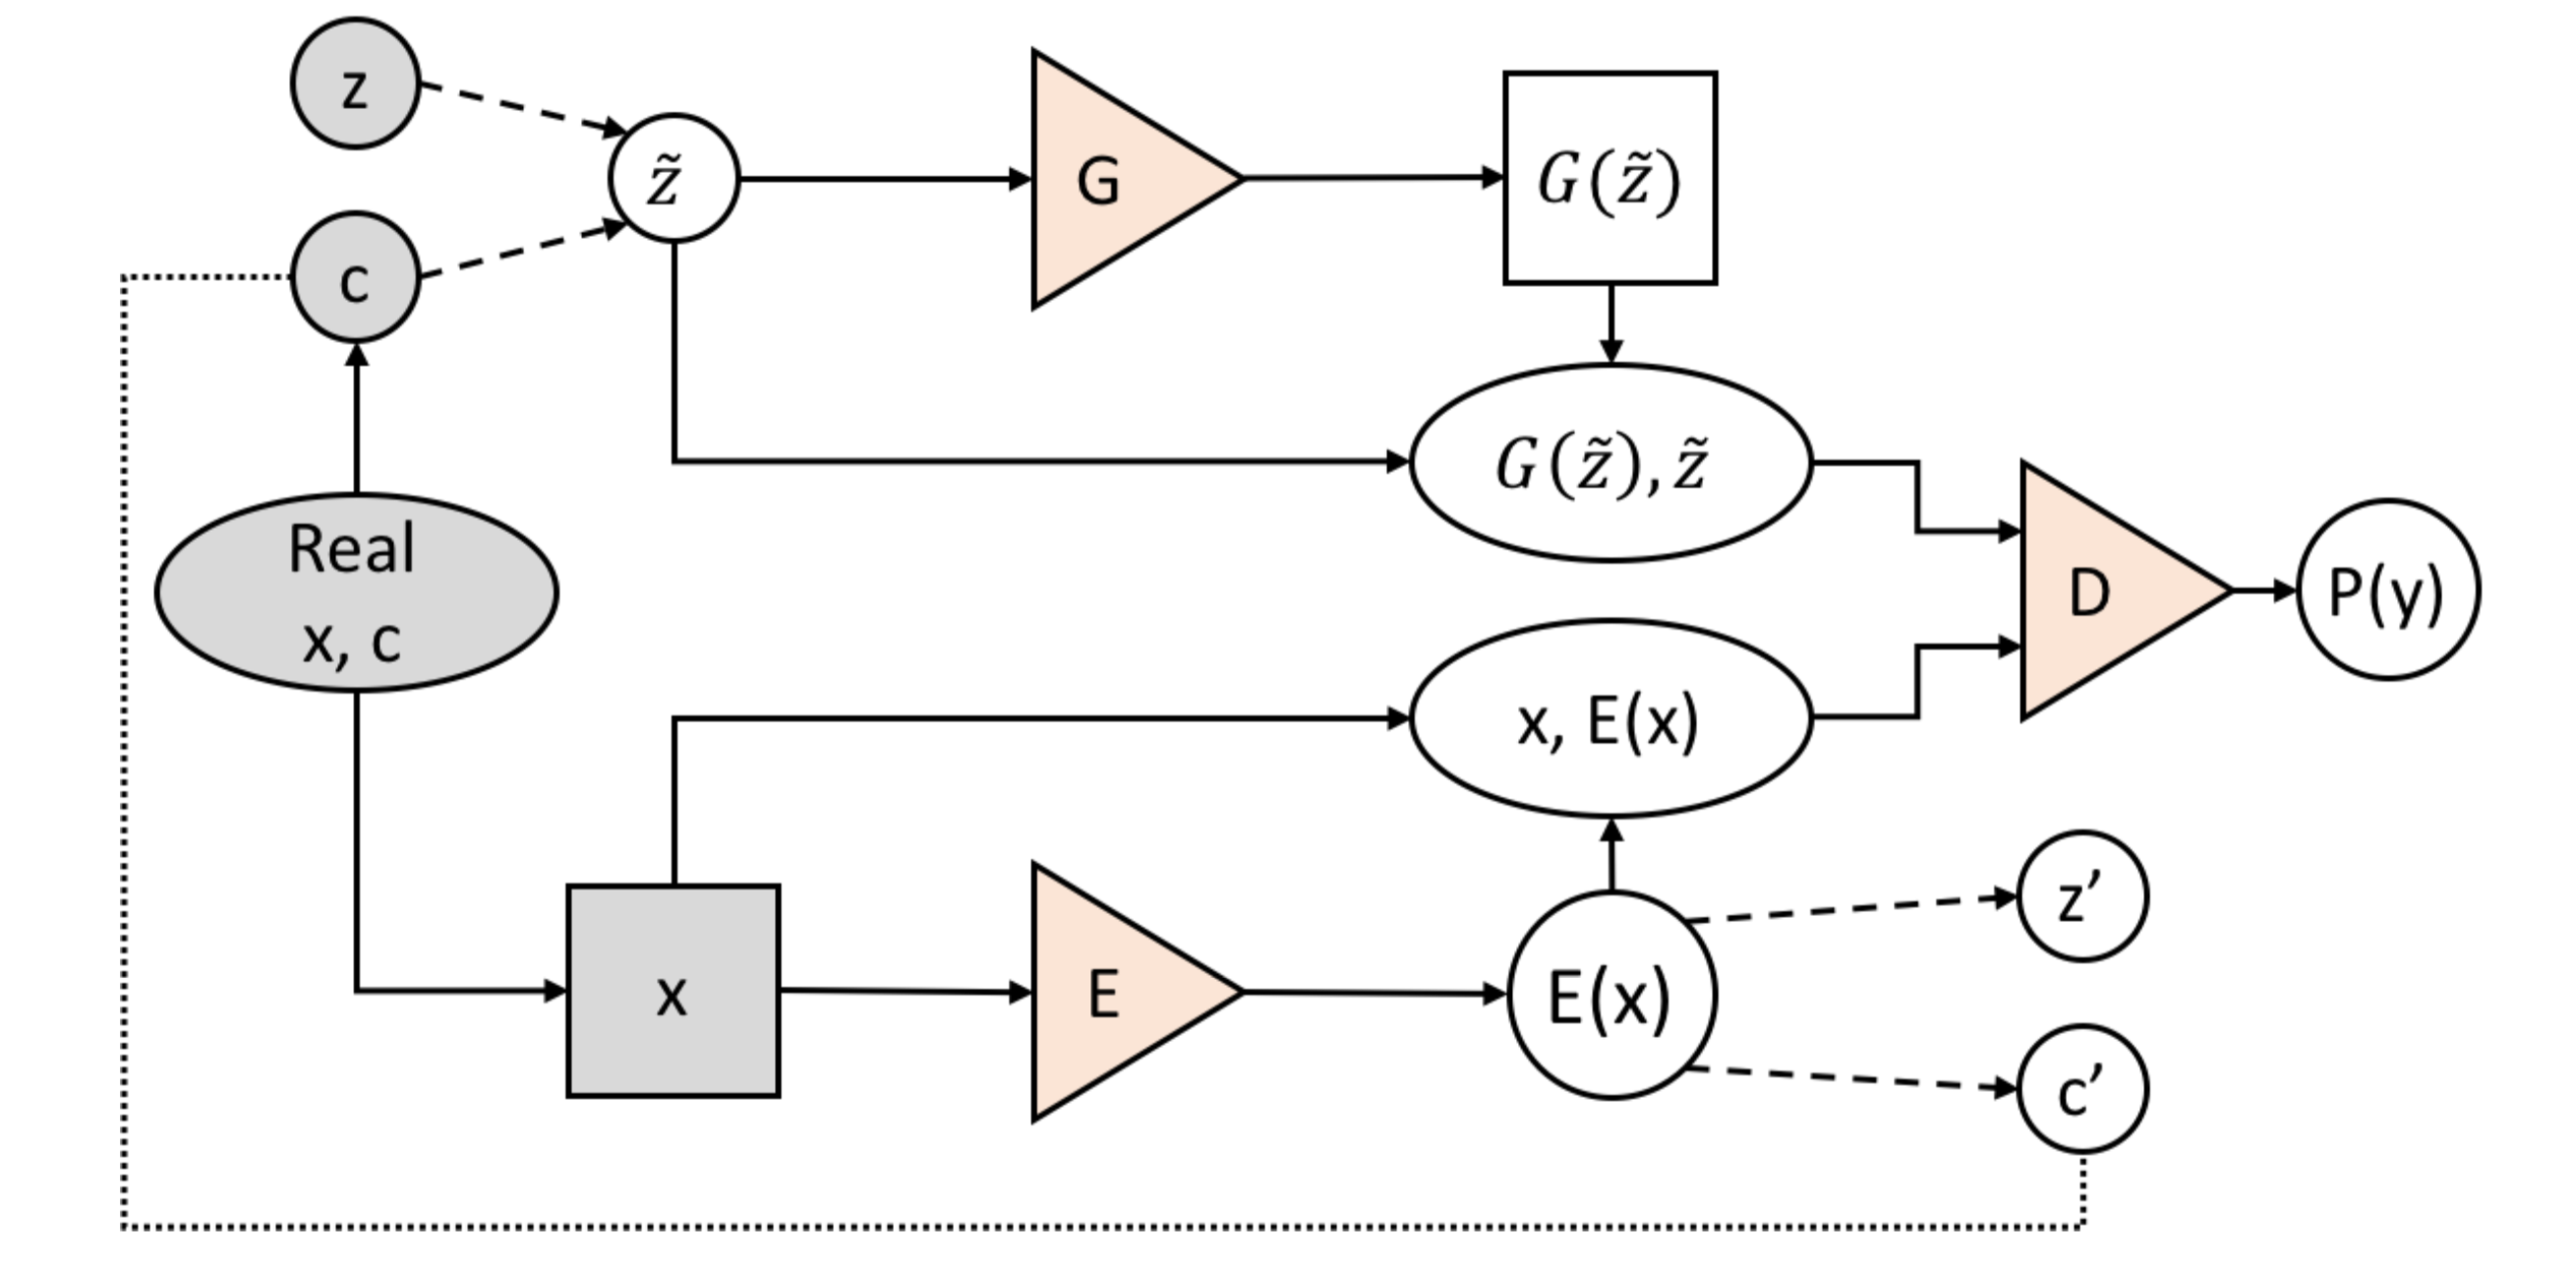
\includegraphics[width=0.7\textwidth]{images/bicogan_shema.png}
 \caption[Idejna zasnova BICOGAN arhitekture, vir: \cite{jaiswal2017bidirectional} ]{Idejna zasnova BICOGAN arhitekture.Vir:\cite{jaiswal2017bidirectional} }
  \label{fig:bicogan-archi}
\end{figure}

Če se nanašamo na oznake, definirane v poglavju o navadnih GAN mrežah, 
potem formalno rečemo, da se generator nauči preslikavo $G(\tilde{z},\theta_G)$ iz porazdelitvne $p_{\tilde{z}}$, kjer je $\tilde{z} = [z \text{ } c]$ v 
porazdelitev $p_G$, kjer je glavni cilj da se $p_G$ in $p_{data}$ čim manj razlikujeta.  Naloga enkoderja $E(x;\theta_E)$ je da slika iz $p_{data}$ v $p_{E}$, kjer želimo da je $p_E$ čim bližje $p_{\tilde{z}}$. Diskriminator  se odloča o avtentičnosti vzorca glede na  $D(\tilde{z},G(\tilde{z});\theta_D)$ in $D(E(x),x;\theta_D)$. 
\\ V splošnem primeru BICOGAN modela  se mora enkoder  naučiti inverzni preslikavo iz $x$ v $z$ \textbf{in} $c$. Ker pa  je to v našem primeru nepotrebno, smo naš model spremenili tako, da je informacija o oznaki $c$ enkoderju vedno podana. 
\subsubsection{Eksperimentalni rezultati}

Poizkusili smo z implementacijo BICOGAN modela v orodju Keras. Kot najenostavnejšo obliko smo za vse tri notranje mreže (diskriminator, generator, enkoder) uporabili polnopovezano arhitekturo. Rezultati, ki smo jih dobili so prikazali solidne vizualne rezultate s strani generatorja, vendar je do težav prišlo pri enkoderju. Ni nam uspelo, da bi se enkoder pravilno naučil preslikave iz $x$ v $z$. Veljati bi namreč moralo, $G(E(x)) \sim  x$, že na prvi pogled pa je očitno, da to ni uspelo. 
\\
Še ena od težav je, da arhitektura s polnopovezanimi sloji generira slike, ki so polne šume in zatorej precej različne od realnih podatkov. 
TBC... 



%
%\section{Uvod}
%
%\section{Integrali po \texorpdfstring{$\omega$}{ω}-kompleksih}
%\subsection{Definicija}
%\begin{definicija}
%  Neskončno zaporedje kompleksnih števil, označeno z $\omega = (\omega_1, \omega_2, \ldots)$,
%  se imenuje \emph{$\omega$-kompleks}.\footnote{To ime je izmišljeno.}
%
%  Črni blok zgoraj je tam namenoma. Označuje, da \LaTeX{} ni znal vrstice prelomiti pravilno
%  in vas na to opozarja. Preoblikujte stavek ali mu pomagajte deliti problematično besedo z
%  ukazom \verb|\hyphenation{an-ti-ko-mu-ta-ti-ven}| v preambuli.
%\end{definicija}
%\begin{trditev}[Znano ime ali avtor]
%  \label{trd:obstoj-omega}
%  Obstaja vsaj en $\omega$-kompleks.
%\end{trditev}
%\begin{proof}
%  Naštejmo nekaj primerov:
%  \begin{align}
%    \omega &= (0, 0, 0, \dots), \label{eq:zero-kompleks} \\
%    \omega &= (1, i, -1, -i, 1, \ldots), \nonumber \\
%    \omega &= (0, 1, 2, 3, \ldots). \nonumber \qedhere  % postavi QED na zadnjo vrstico enačbe
%  \end{align}
%\end{proof}
%
%\section{Tehnični napotki za pisanje}
%
%\subsection{Sklicevanje in citiranje}
%Za sklice uporabljamo \verb|\ref|, za sklice na enačbe \verb|\eqref|, za citate \verb|\cite|. Pri
%sklicevanju in citiranju sklicano številko povežemo s prejšnjo besedo z nedeljivim presledkom
%$\sim$, kot npr.\ \verb|iz trditve~\ref{trd:obstoj-omega} vidimo|.
%
%\begin{primer}
%  Zaporedje~\eqref{eq:zero-kompleks} iz dokaza trditve~\ref{trd:obstoj-omega} na
%  strani~\pageref{trd:obstoj-omega} lahko najdemo tudi v Spletni enciklopediji zaporedij~\cite{oeis}.
%  Citiramo lahko tudi bolj natančno~\cite[trditev 2.1, str.\ 23]{lebedev2009introduction}.
%\end{primer}
%
%\subsection{Okrajšave}
%Pri uporabi okrajšav \LaTeX{} za piko vstavi predolg presledek, kot npr. tukaj. Zato se za vsako
%piko, ki ni konec stavka doda presledek običajne širine z ukazom \verb*|\ |, kot npr.\ tukaj.
%Primerjaj z okrajšavo zgoraj za razliko.
%
%\subsection{Vstavljanje slik}
%Sliko vstavimo v plavajočem okolju \texttt{figure}. Plavajoča okolja \emph{plavajo} po tekstu, in
%jih lahko postavimo na vrh strani z opcijskim parametrom `\texttt{t}', na lokacijo, kjer je v kodi s
%`\texttt{h}', in če to ne deluje, potem pa lahko rečete \LaTeX u, da ga \emph{res} želite tukaj,
%kjer ste napisali, s `\texttt{h!}'. Lepo je da so vstavljene slike vektorske (recimo \texttt{.pdf}
%ali \texttt{.eps} ali \texttt{.svg}) ali pa \texttt{.png} visoke resolucije (več kot
%\unit[300]{dpi}).  Pod vsako sliko je napis in na vsako sliko se skličemo v besedilu. Primer
%vektorske slike je na sliki~\ref{fig:sample}. Vektorsko sliko prepoznate tako, da močno
%zoomate v sliko, in še vedno ostane gladka. Več informacij je na voljo na
%\url{https://en.wikibooks.org/wiki/LaTeX/Floats,_Figures_and_Captions}. Če so slike bitne, kot na
%primer slika~\ref{fig:image}, poskrbite, da so v dovolj visoki resoluciji.
%
%\begin{figure}[h]
%  \centering
%  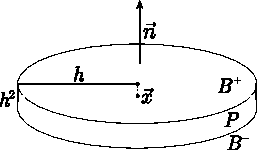
\includegraphics[width=0.6\textwidth]{images/sample.pdf}
%% \caption[caption za v kazalo]{Dolg caption pod sliko}
%  \caption[Primer vektorske slike.]{Primer vektorske slike z oznakami v enaki pisavi, kot jo
%     uporablja \LaTeX{}.  Narejena je s programom Inkscape, \LaTeX{} oznake so importane v
%     Inkscape iz pomožnega PDF.}
%  \label{fig:sample}
%\end{figure}
%
%\begin{figure}[h]
%  \centering
%  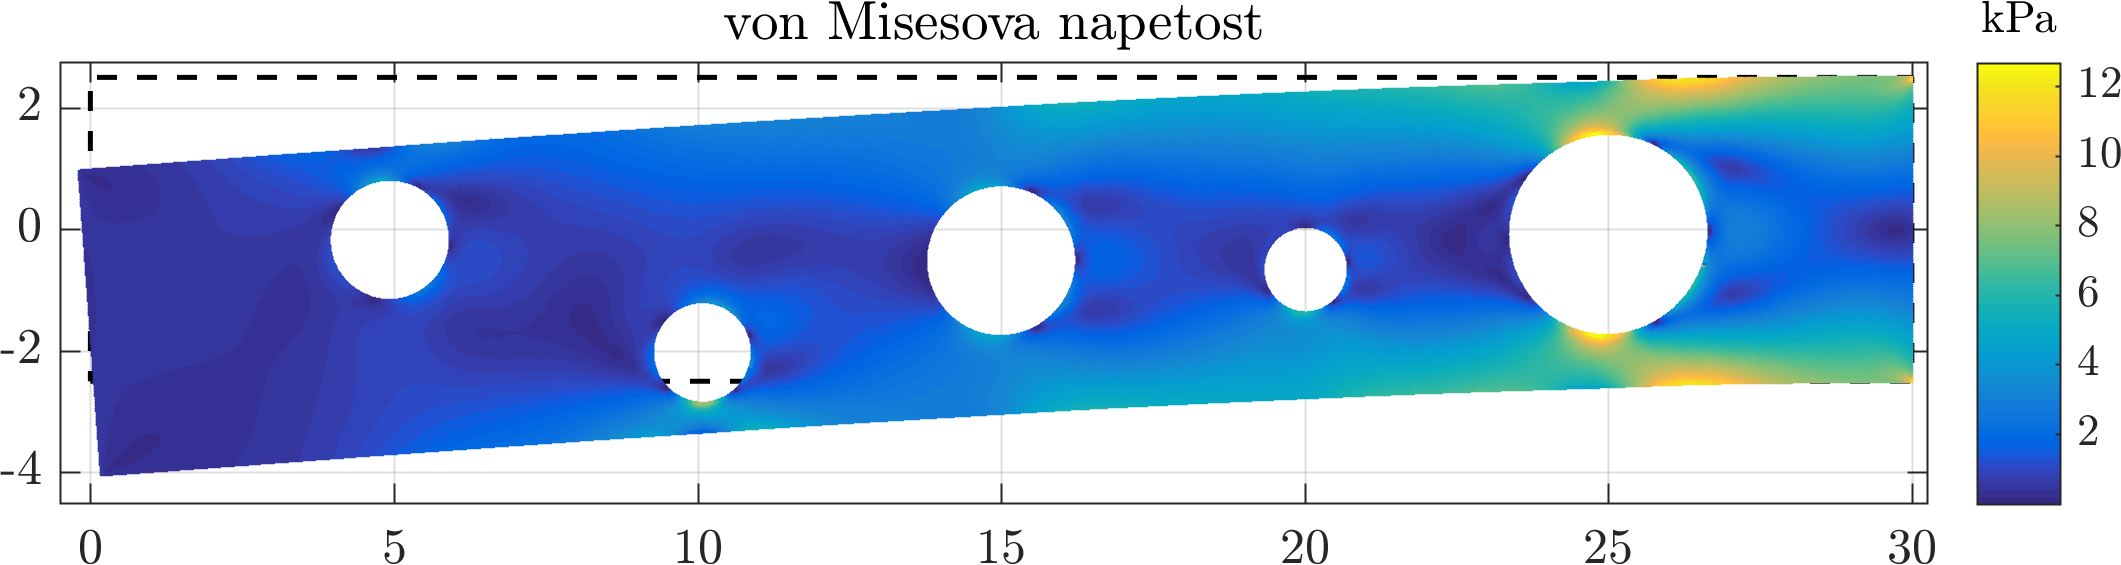
\includegraphics[width=0.8\textwidth]{images/image.png}
%  \caption[Primer bitne slike.]{Primer bitne slike, izvožene iz Matlaba. Poskrbite, da so slike v
%  dovolj visoki resoluciji in da ne vsebujejo prosojnih elementov (to zahteva PDF/A-1b format).}
%  \label{fig:image}
%\end{figure}
%
%\subsection{Kako narediti stvarno kazalo}
%Dodate ukaze \verb|\index{polje}| na besede, kjer je pojavijo, kot tukaj\index{tukaj}.
%Več o stvarnih kazalih je na voljo na \url{https://en.wikibooks.org/wiki/LaTeX/Indexing}.
%
%\subsection{Navajanje literature}
%Članke citiramo z uporabo \verb|\cite{label}|, \verb|\cite[text]{label}| ali pa več naenkrat s
%\verb|\cite\{label1, label2}|. Tudi tukaj predhodno besedo in citat povežemo z nedeljivim presledkom
%$\sim$. Na primer~\cite{chen2006meshless,liu2001point}, ali pa \cite{kibriya2007empirical}, ali pa
%\cite[str.\ 12]{trobec2015parallel}, \cite[enačba (2.3)]{pereira2016convergence}.
%Vnosi iz \verb|.bib| datoteke, ki niso citirani, se ne prikažejo v seznamu literature, zato jih
%tukaj citira m.~\cite{vene2000categorical}, \cite{gregoric2017stopniceni}, \cite{slak2015induktivni},
%\cite{nsphere}, \cite{kearsley1975linearly}, \cite{STtemplate}, \cite{NunbergerTand}.
%
%% Literatura:
%% Primer navajanja na http://www.fmf.uni-lj.si/storage/24240/LiteraturaM.pdf,
%% ampak bi moral stil poskrbeti za vse. Reference se uredijo po abecedi.
%% Če nobena izbira izmed @book, @atricle,... ni ok, potem se lahko vse napiše v
%% @misc pod note={} in deluje tako kot normalen LaTeX.
%% Komentar v bib datoteki se naredi samo s parom { }
%% Za urejanje literature avtor priporoča program Jabref, ki zna tudi avtomatsko
%% okrajšati imena revij. Za pravilno sortiranje vnosov brez avtorja, uporabite
%% polje key={ }, kot v primeru.
%% V primeru napak ustvarite issue na GitHubu ali pišite na jure.slak@fmf.uni-lj.si.
\cleardoublepage                           % na desni strani
\phantomsection                            % da prav delujejo hiperlinki
\addcontentsline{toc}{section}{\bibname}   % dodajmo v kazalo
\bibliographystyle{fmf-sl}                 % uporabljen stil je v datoteki fmf-sl.bst, na voljo tudi angleška verzija
\bibliography{\literatura}                 % literatura je v datoteki, definirani na začetku

% Za stvarno kazalo
\cleardoublepage                           % na desni strani
\phantomsection                            % da prav delujejo hiperlinki
\addcontentsline{toc}{section}{\indexname} % dodajmo v kazalo
\printindex

\end{document}
